\documentclass[10pt,oneside]{amsart}
\usepackage{amsmath}
\usepackage{amsthm}
\usepackage{amsfonts}
\usepackage{amssymb,amscd,epsf,verbatim}
\usepackage{mathrsfs}
\usepackage{graphicx}
\usepackage{latexsym}
\usepackage{standalone}
\usepackage{lscape}
\usepackage{hyperref}
%\usepackage[colorlinks=true]{hyperref}
%\hypersetup{colorlinks, citecolor=blue, filecolor=black, linkcolor=red, urlcolor=green}
\usepackage{epstopdf}
\usepackage{tikz}
\usetikzlibrary{calc}
\usetikzlibrary{matrix,arrows,decorations.pathmorphing}
\usepackage{tikz-cd}
\usepackage{color}
\usepackage{geometry}
\usepackage{multirow}
\usepackage{enumitem}
\usepackage{framed}

\newcommand{\dstyle}{\displaystyle}

%%%%%%% please do NOT add any new command 
%%%%%%(unless it is absolutely necessary, in which case please send everyone an email about it.
%%%%%%%

%\theoremstyle{theorem}
\newtheorem{theorem}{Theorem}[section]
\newtheorem{lemma}[theorem]{Lemma}
\newtheorem{step}[theorem]{step}
\newtheorem{proposition}[theorem]{Proposition}
\newtheorem{corollary}[theorem]{Corollary}
\newtheorem{claim}[theorem]{Claim}
\newtheorem{conjecture}[theorem]{Conjecture}
\newtheorem*{outline}{Outline of Proof}
\newtheorem{mainthm}{Theorem} 
\newtheorem{lemma*}[mainthm]{Lemma}
\newtheorem{proposition*}[mainthm]{Proposition}



\theoremstyle{definition}
\newtheorem{definition}[theorem]{Definition}
\newtheorem{notation}[theorem]{Notation}
\newtheorem{construction}[theorem]{Construction}
\newtheorem{question}[mainthm]{Question}
\newtheorem{remark}[theorem]{Remark}
\newtheorem*{example}{Example}
\newtheorem{remark*}[mainthm]{Remark}
\newtheorem{definition*}[mainthm]{Definition}




\title[perfectoid covers of abelian varieties]{perfectoid  covers of abelian varieties} 
%\date{August 2017}
\author{
	Clifford Blakestad \and
	Dami\'an Gvirtz \and
	Ben Heuer \and 
	Daria Shchedrina \and
	Koji Shimizu \and 
	Peter Wear \and
	Zijian Yao}

\begin{document}
	
	\maketitle
	
	\begin{abstract}
For an abelian variety $A$ over an algebraically closed non-archimedean field of residue characteristic $p$, we show that there exists a perfectoid space which is the tilde-limit of $\varprojlim_{[p]}A$.
	\end{abstract}
	

	
	 %%%%%%%%%%%%
%%      Section 1
%%%%%%%%%%%%
	\section{Introduction} 

Let $p$ be a prime and let $K$ be a non-archimedean field which is either $p$-adic or of characteristic $p$. 
Let us moreover assume that $K$ is algebraically closed. 
For an abelian variety $A$ over $K$ we consider the inverse system of $A$ under the multiplication by $p$ morphism:
\[\dots\xrightarrow{[p]}A\xrightarrow{[p]}A\xrightarrow{[p]}A\]
Via the rigid analytification functor, we may see this as an inverse system of analytic adic spaces over $\operatorname{Spa}(K,\mathcal O_K)$.
The primary goal of this article is to show that the ``inverse limit'' of this tower exists in some way and is a perfectoid space: Since inverse limits rarely exist in the category of adic spaces (even for affinoid spaces), in \cite{SW} the authors introduce the weaker notion of tilde-limits to remedy this problem. This is the notion of "limits" we are going to use. More precisely, we prove:

 %Before we state the precise version of the theorem, we remark that the main assertion already implicitly appeared in [?] [?] without justification. Nevertheless we decide to fill in this gap in the literature, since the proof, despite being straight-forward, is quite subtle to spell out. 
 


\begin{mainthm} \label{thm:main_thm_intro}
	Let $A$ be an abeloid variety over $K$, for instance an abelian variety seen as a rigid space. Then there is a unique perfectoid space $A_\infty$ over $K$ such that
	$A_\infty \sim \varprojlim_{[p]} A$ is a tilde-limit.
\end{mainthm}

The possibility of results in this direction is mentioned in \S 7 and \S 13 of \cite{scholzeICMproceedings}, and in the case of abelian varieties $A$ with good reduction, this theorem was proven already in \cite{Pilloni-Stroh} (Lemme A.16).  In order to motivate our strategy for the general case, let us sketch the proof in the good reduction case (we follow Exercise 4 -- 6 in \cite{Bhatt}, the proof is spelt out in detail in \S \ref{subsection:perfectoid_tilde_limit}, Corollary \ref{tilde-limit exists and is perfectoid in the good reduction case} below):

Let $A$ be an abelian variety of good reduction over $K$. Let $\mathcal O_K$ be the ring of integers of $K$ and let $\pi\in\mathcal O_K$ be a pseudo-uniformiser such that $p\in \pi\mathcal O_K$. Then we can consider $A$ as an abelian scheme over $\mathcal O_K$. Let $\mathcal A$ be its $\pi$-completion, a formal scheme over $\mathcal O_K$. Its adic generic fibre is the rigid analytification of $A$ that we denote by the same letter. The mod $\pi$ special fibre $\mathcal A_s = \mathcal A \times \mathcal O_K/\pi$ is a group scheme over $\mathcal O_K/\pi$, so the map $[p]:\mathcal A_s\rightarrow \mathcal A_s$ factors through the relative Frobenius map. The inverse limit $ \varprojlim_{[p]} \mathcal A_s $ in the category of schemes is thus relatively perfect over $\mathcal O_K/\pi$. We can similarly form the inverse limit $\mathcal A_{\infty} = \varprojlim_{[p]} \mathcal A$ in the category of formal schemes. Its adic generic fibre $A_\infty$ is a tilde-limit of $\varprojlim_{[p]}A$, and it is perfectoid since $ \varprojlim_{[p]} \mathcal A_s $ is relatively perfect.

This gives the construction of $A_\infty$ in the case of good reduction. The overall strategy of our proof of Theorem \ref{thm:main_thm_intro} is similar: We construct tilde-limits of various spaces via formal models and show that these tilde-limits are perfectoid via a Frobenius factorisation property on the special fibre. 

Next, we consider the case that $A$ is an abelian variety with bad reduction. The assumption that $K$ is algebraically closed assures that $A$ is then semi-stable.
In this case, the theory of Raynaud extensions provides us with a short exact sequence 
\[ 0 \rightarrow T \rightarrow E  \rightarrow  B  \rightarrow  0\]
of rigid groups, where $T = (\mathbb G_m^{\text{an}})^{d}$ is a split rigid torus and $B$ is the analytification of an abelian variety with good reduction, such that $A = E/M$ for a discrete lattice $M \subset E$. This short exact sequence is split locally on $B$, allowing us to locally write $E$ as a product of $T$ and an open subspace of $B$.
Our strategy, which more generally applies to any abeloid variety over $K$, is now the following:
\begin{enumerate}
\item Use formal models to show that there exists a perfectoid tilde-limit $T_\infty\sim\varprojlim_{[p]} T$.
\item Use the formal models from (1) to construct a perfectoid tilde-limit $E_\infty\sim\varprojlim_{[p]} E$.
\item Study the quotient map $E\rightarrow A$ in the limit over $[p]$ to construct the desired space $A_\infty$.
\end{enumerate}

More precisely, this article is organised as follows: In \S2 we develop a notion of a $[p]$-$F$-formal tower for a commutative rigid group $G$ over $K$, which is roughly an inverse system of formal models for $[p]:G\rightarrow G$ that factor through the relative Frobenius mod $\pi$. This is an axiomatisation of the data that one uses to construct $A_\infty$ in the case of good reduction. In particular, the same proof shows that if $G$ admits $[p]$-$F$-formal tower, then there is a unique perfectoid tilde-limit $G_\infty \sim  \varprojlim_{[p]} G$.
 
In chapter \S3 we give a $[p]$-$F$-formal tower for a  split rigid torus $T$ in terms of a family of formal models $\mathfrak T_{q^{1/n}}$, thus showing that a perfectoid tilde-limit $T_\infty$ of the inverse system of $[p]$ on $T$ exists. Crucially, this tower of formal models has the extra structure of an action by the formal torus $\overline{T}$.
 
We can therefore in \S4 use the language of formal fibre bundles to construct a  $[p]$-$F$-formal tower for $E$: The Raynaud extension of $A$ arises from a short exact sequence of formal group schemes
\[0\rightarrow \overline{T}\rightarrow \overline{E}\rightarrow B\rightarrow 0\]
by taking generic fibres and forming the pushout with respect to the open immersion $\overline{T}_\eta\rightarrow T$. Equivalently, since the sequence is locally split, we can see $\overline{E}\rightarrow B$ as a principal $\overline{T}$-bundle and formation of $E$ amounts to a change of fibre from $\overline{T}_\eta$ to $T$. Since the formal model tower of \S3 receives a $\overline{T}$-action, we now obtain a $[p]$-$F$-formal tower for $E$ from the formal models of $\S 4$ by the change of fibre from $\overline{T}$ to the formal models $\mathfrak T_{q^{1/n}}$. This gives the desired perfectoid tilde-limit $E_\infty$.

In chapter \S5 we finish the proof of the main theorem by constructing $A_\infty$ from $E_\infty$ as follows: After choosing lattices $M\subseteq M^{1/p^n}\subseteq E$ that are sent to $M$ under $[p^n]:E\rightarrow E$, the $[p]$-multiplication tower of $A=E/M$ naturally factors into two separate towers: One is the tower of maps $E/M^{1/p^{n+1}}\rightarrow E/M^{1/p^{n}}$ induced from $[p]$-multiplication of $E$, the other is induced from the projection maps $E/M\rightarrow E/M^{1/p^n}$. By choosing certain charts of $E$ that give local splittings of the projection $E\rightarrow E/M=A$, we show that the first of these towers has a perfectoid tilde-limit $E/M^{1/p^\infty}$ that is locally isomorphic to open subsets of $E_\infty$. Since the second tower is easy to describe in terms of the chosen charts, it is then straightforward to find the desired space $A_\infty$.
 
In chapter \S6 we finally use our explicit construction to say something about the local geometry of $A_\infty$. In particular, we describe the perfectoid group homomorphism $E_\infty \rightarrow A_\infty$ in terms of perfectoid principal bundles. The goal of this last section is to give an alternative description of $A_\infty$ in terms of a quotient of perfectoid groups: There are a lattice $M_{\infty}\subseteq E_\infty$ and a pro-finite perfectoid group $D_\infty$ over $K$ for which there is a short exact sequence of perfectoid groups
\[0\rightarrow M_\infty\rightarrow D_\infty \times E_\infty \rightarrow A_\infty\rightarrow 0.\]
This may be seen as an analogue in the limit of the sequence $0\rightarrow M\rightarrow E\rightarrow A\rightarrow 0$.

At the end there is an appendix on fibre bundles and associated fibre bundle constructions in the context of formal, rigid and perfectoid spaces.

 \begin{comment}
Now we end the introduction by describing the content of each section. 

	\begin{question} \label{question_intro}
	    \begin{enumerate} 
	    \item		Given a rigid group $G$, when is there an adic space $G_\infty$ such that $G_\infty \sim  \varprojlim_{[p]} G ?$
	    \item If it exists, and $K$ is perfectoid, when is $G_\infty$ perfectoid?
	    \end{enumerate}
	\end{question}
 
 
	But before we give proofs for examples of rigid groups $G$ for which a perfectoid tilde-limit exists, we first note that the second question certainly doesn't have an affirmative answer for all rigid group varieties:
	\begin{example}
		For the additive group $\mathbb G_a^{\operatorname{an}}$, we know that $[p]$ is an isomorphism and therefore $\varprojlim_{[p]} \mathbb G_a=\mathbb G_a$ exists (even as an actual limit in the category of adic spaces) but is certainly not perfectoid.
	\end{example}

\end{comment} 
 
 
 
 \addtocontents{toc}{\protect\setcounter{tocdepth}{0}} %some hack to hide the acknowledgements in the toc
 \section*{Acknowledgements}
 \addtocontents{toc}{\protect\setcounter{tocdepth}{2}} % end hack
 This work started as a group project at the 2017 Arizona Winter School. We would like to thank Bhargav Bhatt for proposing the project, for his guidance and for his constant encouragement, and we would like to thank Matthew Morrow for his help during the Arizona Winter School. In addition we would like to thank the organizers of the Arizona Winter School for setting up a great environment for us to participate in this project. 
 
 During this work Dami\'an Gvirtz and Ben Heuer were supported by the Engineering and Physical Sciences Research Council [EP/L015234/1], the EPSRC Centre for Doctoral Training in Geometry and Number Theory (The London School of Geometry and Number Theory), University College London. 
 During the Arizona Winter School, Daria Shchedrina was supported by Prof. Dr. Peter Scholze and the DFG.
 Peter Wear was supported by NSF grant DMS-1502651 and UCSD and would like to thank Kiran Kedlaya for helpful discussions.


\addtocontents{toc}{\protect\setcounter{tocdepth}{0}} %some hack to hide the acknowledgements in the toc
\section*{Notation}
\addtocontents{toc}{\protect\setcounter{tocdepth}{2}} % end hack
	We fix a prime $p$.  Let $K$ be a perfectoid field that is either $p$-adic or of characteristic $p$, with ring of integers  $\mathcal O_K$ and  a fixed pseudo-uniformiser $\pi\in \mathcal O_K$ such that $p\in\pi\mathcal O_K$.
	From \S4 on we are going to assume that $K$ is algebraically closed, but we don't need to make this assumption yet.
	
	By an adic space over $\operatorname{Spa}(K,\mathcal O_K)$, we mean an adic spaces in the sense of \cite{SW}, and we adopt the notion of perfectoid spaces defined in \S2 \textit{\small ibid}. In their language, adic spaces in the sense of Huber are referred to as \textit{honest} adic spaces. Throughout the article, we make no distinction between rigid spaces and their corresponding honest adic spaces.
	In particular, by a cover of a rigid space we shall always mean a cover of the associated adic space, and therefore the cover of the rigid space will automatically be an admissible cover in the sense of rigid analytic geometry. 
	%{\color{red} I don't understand what this remark means. } The adification functor from rigid to adic is really well-behaved: Open immersions go to open immersions, and a set-theoretic cover by open rigid subspaces is admissible if and only if the induced open immersions of the associated adic spaces give rise to a set-theoretic cover of the adic space. See for instance \S 16 of Conrad's perfectoid seminar, available at http://math.stanford.edu/~conrad/Perfseminar/Notes/L16.pdf
	If a rigid space is obtained from a $K$-scheme $X$ via rigid-analytification $X\mapsto X^{\operatorname{an}}$, we will often denote both by the same symbol $X$ in order to simplify the notation.
	
	In a similar spirit, we are often going to see formal schemes as adic spaces via the fully faithful adification functor, and denote both by the same letter. 
	% I am reluctant to say that we make no distinction between formal schemes and their associated adic spaces, since I think this is much more dangerous for formal schemes than for rigid spaces. For instance, there are morphisms which are open immersions as adic spaces but not as formal schemes, for formal completions the morphisms of the underlying locally ringed spaces are substantially different, etc etc.
	For a formal scheme $\mathfrak X$ over $\operatorname{Spf}(\mathcal O_K)$ with the $\pi$-adic topology, we denote by $\mathfrak X_\eta:=\mathfrak X\times_{\operatorname{Spa}(\mathcal O_K,\mathcal O_K)}\operatorname{Spa}(K,\mathcal O_K)$ its adic generic fibre. 
	We denote by $\tilde{X}=\mathfrak X\times_{\operatorname{Spf}\mathcal O_K}\operatorname{Spf}\mathcal O_K/\pi$ its mod $\pi$ special fibre, considered as a scheme over $\operatorname{Spec}\mathcal O_K/\pi$. 

	Finally, let us recall the following standard terminology: 
		\begin{enumerate}
			\item Let $X$ be a rigid space over $K$. A \textbf{formal model} of $X$ is an admissible topologically finite type formal scheme $\mathfrak X$ over $\mathcal O_K$ together with an isomorphism of its generic fibre $\mathfrak X_\eta \xrightarrow{\sim} X$ (which is often suppressed from notation).
			\item Let $\phi:  X\rightarrow  Y$ be a morphism of rigid spaces over $K$, with formal models $\mathfrak X$ and $\mathfrak Y$	respectively. A morphism of formal schemes $\Phi:\mathfrak X \rightarrow \mathfrak Y$ is a \textbf{formal model} of $\phi$ if it agrees with $\phi$ on the adic generic fiber via the identifications $\mathfrak X_\eta \xrightarrow{\sim} X$ and $\mathfrak Y_\eta \xrightarrow{\sim} Y$.
		\end{enumerate}


%%%%%%%%%%%%
%%      Section 2
%%%%%%%%%%%%	
	
\numberwithin{theorem}{section}
	\section{Tilde-limits of rigid groups} \label{section:tilde_limit}
  
	

		\subsection{Tilde-limits and formal models} 
		
	Inverse limits often do not exist in the category of adic spaces, and neither do they in rigid spaces. Instead we use the notion of tilde-limits from \cite{SW}:
	
	\begin{definition} 
Let $(X_i)_{i\in I}$ be a filtered inverse system of adic spaces with quasi-compact and quasi-separated transition maps, let $X$ be an adic space with a compatible system of morphisms $f_i: X \rightarrow X_i$. We write $X \sim \varprojlim X_i$ and say that $X$ is a \textbf{tilde-limit} of the inverse system $(X_i)_{i\in I}$ if the map of underlying topological spaces $|X| \rightarrow \varprojlim |X_i|$ is a homeomorphism, and there exists an open cover of $X$ by affinoids $\operatorname{Spa} (A, A^+) \subset X$ such that the map 
$$ \varinjlim_{\operatorname{Spa}(A_i, A_i^+) \subset X_i} A_i \rightarrow A$$
has dense image, where the direct limit runs over all $i\in I$ and all open affinoid subspaces $\operatorname{Spa}(A_i, A_i^+) \subset X_i$ through which the morphism $\operatorname{Spa}(A, A^+) \subseteq X\rightarrow X_i$ factors.
	\end{definition}
	
	\begin{remark} \label{remark:tilde_limit_non_unique}
As pointed out after Proposition 2.4.4 of \cite{SW}, tilde-limits (if they exist) are in general not unique. For example, consider the inverse system consisting of a single affinoid pre-perfectoid space $X = \operatorname{Spa}(A, A^+)$ in the sense of Definition~2.3.4 in \cite{SW}. Then both the space $X$ as well as its strong completion $\hat X = \operatorname{Spa}(\hat A,\hat A^+)$ are tilde-limits of $X$. However, we'll see in Corollary~\ref{corollary: perfectoid tilde limit is unique} that the perfectoid tilde-limits we construct are unique.
	\end{remark}

Let us recall a few results from \cite{SW}, \S2.4 about the construction of tilde-limits that we will use frequently throughout:

\begin{proposition}[\cite{SW}, Proposition 2.4.2]\label{SW Proposition 2.4.2}
	Let $(A_i,A_i^{+})$ be a direct system of affinoids over $(\mathcal O_K,\mathcal O_K)$ with compatible rings of definition $A_{i,0}$ carrying the $\pi$-adic topology. Let $(A,A^{+})=(\varinjlim A_i,\varinjlim A_i^{+})$ be the affinoid algebra equipped with the topology making $\varinjlim A_{i,0}$ with the $\pi$-adic topology a ring of definition. Then
	\[\operatorname{Spa}(A,A^{+})\sim \varprojlim \operatorname{Spa}(A_i,A_i^{+}).\]
\end{proposition}
\begin{proposition}[\cite{SW}, Proposition 2.4.3]\label{SW Proposition 2.4.3}
	Let $X\sim \varprojlim_{i\in I} X_i$ be a tilde-limit and let $U_i\hookrightarrow X_i$ be an open immersion for some $i\in I$. Let $U_j:=U_i\times_{X_i}X_j$ for $j\geq i$ and $U:=U_i\times_{X_i}X$, then 
	\[U\sim \varprojlim_{j\geq i} U_j.\]
\end{proposition}

\begin{proposition}[\cite{SW}, Proposition 2.4.5]\label{SW Proposition 2.4.5}
	Let $(X_i)_{i\in I}$ be an inverse system of adic spaces over $(K,\mathcal O_K)$ and assume that there is a perfectoid space $X$ such that $X\sim \varprojlim_{i\in I} X_i$. Then for any perfectoid $(K,\mathcal O_K)$-algebra $(B,B^{+})$, 
	\[X(B,B^{+})  = \varprojlim_{i\in I}X_i(B,B^{+})\]
\end{proposition}
\begin{corollary}\label{corollary: perfectoid tilde limit is unique}
	If a perfectoid tilde-limit $X\sim \varprojlim X_i$ exists, it is unique up to unique isomorphism.
\end{corollary}
In the situation of the Corollary, we will also refer to $X$ as \textit{the} perfectoid tilde-limit of $ \varprojlim X_i$. Of course perfectoid tilde-limit don't always exists. One case in which this they exist is the following:
\begin{proposition}\label{proposition: tilde-limits of perfectoid spaces}
	Let $(\operatorname{Spa}(A_i,A_i^{+}))_{i\in I}$ be an inverse system of affinoid perfectoid spaces over $(K,\mathcal O_K)$. 
	Let $(A,A^{+}) = (\varinjlim A_i,\varinjlim A_i^{+})$ be the affinoid algebra endowed with the topology making $A_0=\varinjlim A_i^{\circ}$ with the $\pi$-adic topology an open subring of definition, and denote by $(\hat{A},\hat{A}^+)$ the completion. Then $\operatorname{Spa}(A,A^{+})\sim \varprojlim \operatorname{Spa}(A_i,A_i^{+})$ is a perfectoid tilde-limit.
\end{proposition}
\begin{proof}
	The space $\operatorname{Spa}(A,A^{+})$ is a tilde-limit of $(A,A^{+})$ by Proposition~\ref{SW Proposition 2.4.2}. It is then clear from the definition that this remains true for $(\hat{A},\hat{A}^{+})$. It remains to see that this is a perfectoid $(K,\mathcal O_K)$-algebra: But $\hat{A_0}$ is a flat $\mathcal O_K$-algebra and in the direct limit the Frobenius isomorphisms $A_i^{\circ}/\pi^{1/p}\cong A_i^{\circ}/\pi$ induce an isomorphism
	\[\hat{A_0}/\pi^{1/p}\cong \hat{A_0}/\pi.\]
	Thus by Lemma~5.6 in \cite{perfectoid}, $(\hat{A},\hat{A}^+)$ is a perfectoid $(K,\mathcal O_K)$-algebra. 
\end{proof}
	

In the situation that the $X_i$ are rigid space, one way to construct tilde-limits is by constructing well-behaved formal models. The reason for this is the combination of the following two Lemmas:

	\begin{lemma} \label{lemma:inverse_limit_formal}
		Let $(\mathfrak X_i,\phi_{ij})_{i\in I}$ be an inverse system of formal schemes $\mathfrak X_i$ over $\mathcal O_K$ with affine transition maps $\phi_{ij}:\mathfrak X_j\rightarrow \mathfrak X_i$. Then the inverse limit $\mathfrak X=\varprojlim \mathfrak X_i$ exists in the category of formal schemes over $\mathcal O_K$. If all the $\mathfrak X_i$ are flat formal schemes, so is $\mathfrak X$.
	\end{lemma}
	\begin{proof}
	In the affine case, if the inverse system is $\operatorname{Spf} A_i$, take $A$ to be the $\pi$-adic completion of $\varinjlim A_i$, then  $\operatorname{Spf} A$ is the inverse limit of the $\operatorname{Spf}A_i$. If the $A_i$ are flat, then so is $A$ because it is torsion-free over the valuation ring $\mathcal O_K$. 
	
	In general, ones uses that the transition maps are affine to reduce to the affine case. 
	\end{proof}
	
	The proof also shows that in the situation of the Lemma, $\mathfrak X$ is in particular a tilde-limit  $\mathfrak X\sim \varprojlim \mathfrak X_i$ when considered as adic spaces. This remains true after passing to adic generic fibres:
	
	\begin{lemma}\label{tilde-limit from adic generic fibre of formal schemes}
		Let $(\mathfrak X_i,\phi_{ij})_{i\in I}$ be an inverse system of formal schemes $\mathfrak X_i$ over $\mathcal O_K$ with affine transition maps $\phi_{ij}$ and let $\mathfrak X=\varprojlim_{\phi_j} \mathfrak X_i$ be the limit. Let $\mathcal X_i =(\mathfrak X_i)_\eta$ and  $\mathcal X = (\mathfrak X)_\eta$ be the adic generic fibres. Then $\mathcal X \sim \varprojlim \mathcal X_i$.
	\end{lemma}
	\begin{proof}
		This is a consequence of Proposition~\ref{SW Proposition 2.4.2}: The transition maps in the system are affine, hence quasi-compact quasi-separated. In order to prove the Lemma, we can restrict to an affine open subset $\operatorname{Spf}(A)$ of $\mathfrak X$ that arises as the inverse limit of affine open subsets $\operatorname{Spf}(A_i)\subseteq \mathfrak X_i$. Here all formal schemes are considered with the $\pi$-adic topology and $A$ is the $\pi$-adic completion of $\varinjlim A_i$. 
		On the generic fibre, $A_i$ with the $\pi$-adic topology is an open subring of definition of $A_i[1/\pi]$. Therefore, Proposition~\ref{SW Proposition 2.4.2} applies and shows that $\operatorname{Spf}(A)_\eta \sim \varprojlim \operatorname{Spf}(A_i)_\eta$ as desired.
	\end{proof}
	
	\begin{remark}
	This lemma essentially says that one can always construct a tilde-limit of an inverse system of rigid spaces $\mathcal X_i$ if it arises from an inverse system of formal schemes $\mathfrak X_i$ with affine transition maps. This is precisely what Scholze uses in \cite{torsion} to construct the space $\mathcal X_{\Gamma_0(p^\infty)}(\epsilon)_a$ (see Corollary III.2.19 in \cite{torsion} and its proof).
	\end{remark}
	
	%Therefore, one way to construct  a tilde-limit $\varprojlim \mathcal X_i$ for an inverse system of rigid spaces $\mathcal X_i$ is to look for formal models $\mathfrak X_i$ of the system with affine transition maps. If such data exist, Lemma~\ref{tilde-limit from adic generic fibre of formal schemes} produces a tilde-limit $\mathcal X \sim \varprojlim \mathcal X_i$. 
	
 	\begin{remark} \label{Raynaud theory main theorem}
			
	Let us recall Raynaud's theory of formal models: Under mild assumptions,
	one can always find formal models of rigid spaces, and (possibly after admissible blow ups) of morphisms between them. More precisely, Raynaud's theorem \cite[section 8.4]{Bosch lectures} states that
		
		\begin{enumerate}
			\item Let $X$ be a quasi-separated quasi-paracompact rigid space over $K$. Then there exist an admissible quasi-paracompact formal model $\mathfrak X$ for $X$.
			\item If $\mathfrak X'\rightarrow \mathfrak X$ is an admissible blow-up of admissible formal schemes, then it induces an isomorphism on the generic fibre  $\mathfrak X'_\eta \xrightarrow{\sim} \mathfrak X_\eta$.
			\item Let $\mathfrak X$ and $\mathfrak Y$ be admissible quasi-paracompact formal schemes over $\mathcal O_K$ and let $f:\mathfrak X_\eta \rightarrow \mathfrak Y_\eta$ be a morphism of their associated rigid spaces. Then there exist an admissible blow-up $\pi:\mathfrak X'\rightarrow \mathfrak X$ and a map $\mathfrak f:\mathfrak X'\rightarrow \mathfrak Y$ such that $\mathfrak f_\eta = f\circ \pi_\eta$.
		\end{enumerate}
		In particular, given an inverse system ($\mathcal X_i,\phi_{ij})$ of rigid spaces, one can always choose formal models $\mathfrak X_i$ for the $\mathcal X_i$, and by successive admissible blow-ups one can also find models for the transition maps $\phi_{ij}$. This theorem doesn't immediately allow us to construct a tilde-limit using Lemma \ref{tilde-limit from adic generic fibre of formal schemes} as the morphisms might not be affine.
		\end{remark}
		
We will need the following basic lemma later on.

	\begin{lemma}\label{affinoid tilde-limits commute with fibre products}
		Let $(A_i, A_i^+)$ and $(B_i, B_i^+)$ be direct systems of affinoids over $(K, \mathcal O_K)$ with compatible rings of definition $A_{i,0}$ and $B_{i,0}$ carrying the $\pi$-adic topology. Let $\operatorname{Spa}(A, A^+)\sim \varinjlim \operatorname{Spa}(A_i, A_i^+)$ and $\operatorname{Spa}(B, B^+)\sim \varinjlim \operatorname{Spa}(B_i, B_i^+)$ (note that we are not necessarily using the tilde-limits constructed in Proposition \ref{SW Proposition 2.4.2}). Then \[\operatorname{Spa}(A, A^+)\times\operatorname{Spa}(B, B^+)\sim\varprojlim (\operatorname{Spa}(A_i, A_i^+)\times \operatorname{Spa}(B_i, B_i^+))\]
	\end{lemma}
	
	\begin{proof}
		The map of underlying topological spaces is a homeomorphism as fibre products of topological spaces commute with inverse limits. We are therefore reduced to checking that if $\varinjlim A_i \rightarrow A$ has dense image and $\varinjlim B_i \rightarrow B$ has dense image, then $\varinjlim (A_i\otimes B_i) \rightarrow A\otimes B$ has dense image. As direct limits commute with tensor products, we have $\varinjlim (A_i\otimes B_i) = (\varinjlim A_i)\otimes (\varinjlim B_i)$. Now density can be checked directly on elements. 
	\end{proof}
	
	As local tilde-limits glue, the above lemma instantly extends to the case where our tilde-limits come from the setup of Lemma \ref{tilde-limit from adic generic fibre of formal schemes}.
	
\subsection{Tilde-limits for rigid groups}

Let $G$ be a rigid group over $K$, that is, a group object in the category of rigid spaces over $K$. Throughout we will always consider commutative rigid groups. The main topic of study of this work is the $[p]$-multplication tower
\[ \dots\xrightarrow{[p]}G\xrightarrow{[p]}G.\]
\begin{question}
	When is there a perfectoid space $G_\infty$ such that $G_\infty \sim \varprojlim_{[p]} G$ is a tilde-limit?
\end{question}
We are primarily interested in the following examples:
\begin{enumerate}	 
\item Analytifications of finite type group schemes over $K$. Examples include the analytification of an abelian variety $A$ over $K$ and of tori $T$ over $K$.
\item Generic fibres of topologically finite type formal group schemes over $\mathcal O_K$.
\item Raynaud's covering space $E$  of an abelian variety with semi-stable reduction.
\end{enumerate}

	Lemma \ref{lemma:inverse_limit_formal} and  \ref{tilde-limit from adic generic fibre of formal schemes} motivate the following definition. 
	\begin{definition}
	Let $G$ be a rigid group. A \textbf{$[p]$-formal tower} for $G$ is  a family of formal models $\{\mathfrak G_n\}_{n\in \mathbb N}$ of $G$, together with affine transition maps $[\mathfrak p]_{n+1}:\mathfrak G_{n+1}\rightarrow \mathfrak G_{n}$ which are formal models of $[p]:G\rightarrow G$. Sometimes we suppress notation and write $[\mathfrak p]$ for $[\mathfrak p]_{n}$ on $\mathfrak G_n$. 
	\end{definition}
	
	The following Corollary is an immediate consequence of our discussion in the previous subsection:
	\begin{corollary}
		Let $G$ be a rigid group. If $G$ admits a $[p]$-formal tower, then there exists an adic space $G_\infty$ such that $G_\infty \sim \varprojlim_{[p]}G$.
	\end{corollary}
	For example, for any formal group scheme $\mathfrak G$ for which $[p]$ is affine, the $[p]$-multiplication tower of $\mathfrak G$ gives rise to a $[p]$-formal tower for its generic fibre $\mathfrak G_\eta$. 
	
	
	
	
	\subsection{Perfectoidness}  \label{subsection:perfectoid_tilde_limit}

We now introduce the formalism of $[p]$-$F$-formal towers to axiomatise the approach mentioned in the introduction which shows that $A_\infty$ exists and is perfectoid in the case of good reduction.
	
	\begin{definition}
		A \textbf{$[p]$-$F$-formal tower} for a rigid analytic group $G$ is a $[p]$-formal tower 
		$$(\{\mathfrak G_n\}_{n\in \mathbb N}, [\mathfrak p]_{n+1}:\mathfrak G_{n+1}\rightarrow \mathfrak G_{n})$$ such that on the mod $\pi$ special fibre  $\tilde{G}_n$, each   $[\mathfrak p]_{n+1}$ factors through the relative Frobenius map:
				\begin{center}
					\begin{tikzcd}
						& \tilde G_{n+1}^{(p)} \arrow[rd, dashed] &  \\
						\tilde G_{n+1} \arrow[rr, "{[\mathfrak p]_{n+1}}"] \arrow[ru, "F_{rel}"] &  & \tilde G_{n}
					\end{tikzcd}
				\end{center}
	 
	\end{definition}	
	
	 	\begin{proposition}\label{existence of p-F-formal tower implies perfectoid}
		Let $G$ be a rigid group over a perfectoid field $K$. If $G$ admits a $[p]$-$F$-formal tower, then there exists a perfectoid space $G_\infty$ such that $G_\infty \sim \varprojlim_{[p]}G$.
	\end{proposition}

	 
	\begin{proof}
		
		Let $(\{\mathfrak G_n\}_{n\in \mathbb N}, [\mathfrak p]_{n+1}:\mathfrak G_{n+1}\rightarrow \mathfrak G_{n})$ be a $[p]$-$F$-formal tower for $G$.  By Lemma~\ref{tilde-limit from adic generic fibre of formal schemes} we have 
		$$G_\infty := (\varprojlim_{[\mathfrak p]}\mathfrak G)_\eta \sim \varprojlim_{[p]}G. $$
 
		
		To see that $G_\infty$ is perfectoid, we proceed as the proof of \cite{torsion}, Corollary III.2.19. It suffices to prove that $\mathfrak G_\infty = \varprojlim_{[\mathfrak p]} \mathfrak G$ can be covered by formal schemes of the form $\operatorname{Spf}(S)$ where $S$ is a flat $\mathcal O_K$-algebra such that the Frobenius map \[S/\pi^{1/p} \rightarrow  S/\pi\] is an isomorphism. Lemma~5.6 of \cite{perfectoid} then shows that $S[1/\pi]$ is perfectoid.
		
		By assumption, on the mod $\pi$ special fibre  $\tilde{G}_n$,  $[\mathfrak p]_{n+1}$ factors through the relative Frobenius. Now take   any affine open subspace $\operatorname{Spf}(S_0) \subseteq \mathfrak G_0$.  Let $[\mathfrak p^i]:   \mathfrak G_i \rightarrow  \mathfrak G_0$ be the composition $[\mathfrak p]_{i} \circ \cdots \circ [\mathfrak p]_{1}$, and let $\operatorname {Spf}S_i \subset \mathfrak G_i$ be the pullback of $\operatorname {Spf}S_0$ via $[p^i]$. Then we have a commutative diagram:
		\begin{center}
			\begin{tikzcd}[row sep = small]
				&  & \tilde{S}_{i}^{(p)} \arrow[rd, "F_{rel}"] &  & \tilde{S}_{i+1}^{(p)} \arrow[rd, "F_{rel}"] &  &  \\
				\dots \arrow[r] & \tilde{S}_{i-1} \arrow[rr] \arrow[ru, "V", dashed] &  & \tilde{S}_i \arrow[ru, "V", dashed] \arrow[rr] &  & \tilde{S}_{i+1} \arrow[r] & \dots
			\end{tikzcd}
		\end{center} where the horizontal maps are induced from $[\mathfrak p] \mod \pi$. 
		
		From this we can check on elements that relative Frobenius is an isomorphism on $\tilde{S}_\infty := \varinjlim_i \tilde{S}_i$. Since $K$ is perfectoid, we moreover have an isomorphism $\mathcal O_K/\pi^{1/p}\rightarrow \mathcal O_K/\pi$ from the absolute Frobenius on $\mathcal O_K/\pi$. Therefore absolute Frobenius on $S_\infty/\pi$ induces an isomorphism
		\[S_\infty/\pi^{1/p}\xrightarrow{\sim} S_\infty/\pi.\]
		Since each $\mathfrak G_i$ is flat, so are the $S_i$ and thus so is $S_\infty$. Thus $S_\infty[1/\pi]$ is a perfectoid $K$-algebra.
		Since $G_\infty$ is covered by affinoids of the form $\operatorname{Spf}(S_\infty)_\eta$, this shows that $G_\infty$ is perfectoid.
	\end{proof}
	
In particular this gives in more detail the proof of the result that we sketched in the introduction:
	\begin{corollary}\label{tilde-limit exists and is perfectoid in the good reduction case}
		Let $A$ be an abelian variety of good reduction over a perfectoid field $K$. Then $A_\infty$ exists and is perfectoid.
	\end{corollary}
	 	
More generally, if $\mathfrak G$ is a flat commutative formal group scheme such that $[p]$-multiplication is affine, then the maps $[p]:\mathfrak G \rightarrow \mathfrak G$ define a $[p]$-$F$-formal tower for the rigid analytic group $G=\mathfrak G_\eta$, and  $G_\infty := (\varprojlim_{[p]}\mathfrak G)_\eta$ is the perfectoid tilde-limit of $\varprojlim_{[p]} G$. 

%\begin{remark} What we aim to prove in the rest of this write-up is that for a Raynaud extension $0\rightarrow T\rightarrow E\rightarrow B\rightarrow 0$, there is a $[p]$-$F$-model for $T$ which induces a $[p]$-$F$-model for $E$. This will prove that tilde-limits $T_\infty$ and $E_\infty$ exist and are perfectoid if $K$ is perfectoid.  
%\end{remark}
		
\subsection{Examples}				
		
	\begin{example}
		Let $\mathfrak G$ be the $p$-adic completion of the affine group scheme $\mathbb G_m$ over $\mathcal O_K$. The underlying formal scheme of $\mathfrak G$ is $\operatorname {Spf} \mathcal O_K\langle X^{\pm 1} \rangle$.  Multiplication by $p$ on $\mathbb G_m$ gives a $[p]$-$F$-formal tower for $G$, so for the generic fibre $G=\mathfrak G_\eta$ we obtain the perfectoid tilde-limit $G_\infty := (\mathfrak G_\infty)_{\eta} \sim \varprojlim_{[p]} G$. More precisely,  multiplication by $p$ corresponds to the homomorphism
		\[[p]:\mathcal O_K\langle X^{\pm 1} \rangle\rightarrow  \mathcal O_K\langle X^{\pm 1} \rangle, \quad X\rightarrow X^{p}.\]
		In the direct limit, we obtain $   (\varinjlim_{[p]} \mathcal O_K\langle X^{\pm 1} \rangle  )^{\wedge} = \mathcal O_K\langle  X^{\pm 1/p^\infty} \rangle$.  Therefore, taking the generic fiber we get
		$$G_\infty = \operatorname{Spa}(K\langle X^{\pm 1/p^\infty} \rangle,\mathcal O_K\langle X^{\pm 1/p^\infty} \rangle)$$
		and one can verify directly that we indeed have $G_\infty \sim \varprojlim_{[p]} G$.
	\end{example}
	
	
	\begin{example}
		An example of a very different flavour is  the $p$-adic completion  $\mathfrak G$  of the affine group scheme $\mathbb G_a$ over $\mathcal O_K$. Note that $G=\mathfrak G_\eta$ is not equal to $\mathbb G_a^{an}$, but is the closed unit disc in the latter.
		
		The underlying formal scheme of $\mathfrak G$ is $\operatorname {Spf} S$ with $S=\mathcal O_K\langle X \rangle$, and the $[p]$-multiplication is now given by
		\[[p]:\mathcal O_K\langle X \rangle\rightarrow  \mathcal O_K\langle X \rangle, \quad X\rightarrow pX.\]
		In the direct limit, we first obtain the algebra $S'_\infty  = \mathcal O_K\langle \frac{1}{p^\infty}X \rangle$, consisting of power series $f=\sum_{n=0}^\infty  a_nX^n\in \mathcal O_K[[X]]$ for which there exists an $m\in \mathbb Z_{\geq 0}$ so that $|p^{nm}a_n|\to 0$. Next we need to take the $p$-adic completion to form $S_\infty$. But we have 
		\[p^n\mathcal O_K\langle \frac{1}{p^\infty}X \rangle = p^n\mathcal O_K + X \mathcal O_K\langle \frac{1}{p^\infty}X \rangle\]
		and therefore $S'_\infty/\pi^n=\mathcal O_K/\pi^n\mathcal O_K$. Consequently, the completion is just $S_\infty = \mathcal O_K$ and thus its adic generic fiber is $G_\infty = \operatorname{Spa}(K,\mathcal O_K)$.  This is still perfectoid but is just one point!
		
		One can explain this observation geometrically: On the level of $K$-points, the formal scheme $G$ is the closed unit disc and $[p]$ is scaling by $p$. A $K$-point in $\varprojlim_{[p]} G(K)$ therefore corresponds to a sequence of $K$-points of the closed unit disc of the form 
		$$(x,\frac{1}{p}x,\frac{1}{p^2}x,\dots).$$ But for this to be contained in the closed unit disc, we must have $x=0$. 
		
	\end{example}
	
 
 
	
 
	
		
	\subsection{group structure of the limit}
	
	One reason why perfectoid limits along group morphisms are particularly interesting is that the perfectoidness ensures that the limit has again a group structure:
	
	\begin{definition}
		A \textbf{perfectoid group} is a group object in the category of perfectoid spaces.
	\end{definition}
	
			Note that the category of perfectoid spaces over $K$ has finite products, so the notion of a group object makes sense. 
	
	\begin{proposition}\label{perfectoid tilde-limit is perfectoid group in a functorial way}
		Let $G$ be a rigid group with a perfectoid tilde-limit $G_\infty\sim \varprojlim_{[p]}G$. Then
		\begin{enumerate}
		\item  there is a unique way to endow $G_\infty$ with the structure of a perfectoid group in such a way that all projections $G_\infty\rightarrow G$ are group homomorphisms
		\item given another rigid group $H$ with perfectoid tilde-limit $H_\infty\sim\varprojlim_{[p]}H$ and a group homomorphism $H\rightarrow G$, there is a unique group homomorphism $H_\infty\rightarrow G_\infty$
		commuting with all projection maps. In particular, formation of the perfectoid $\varprojlim_{[p]}$ is functorial.
	\end{enumerate}
	\end{proposition}
	\begin{proof}
		These are all consequences of the universal property of the perfectoid tilde-limit, Proposition~\ref{SW Proposition 2.4.5}, which shows that one can argue like in the case of usual limits.
	\end{proof}


  %%%%%%%%%%%%
%%      Section 3
%%%%%%%%%%%%	
	\section{Formal models for tori}
	
	In this section we want to show that for a split rigid torus $T$ over $K$, a tilde-limit $T_\infty$ exists and is perfectoid. We do this by exhibiting a $[p]$-$F$-model of $T$.
	
	As a preparation, we consider the torus $\mathbb G_m^{\operatorname{an}}$ over $K$. Recall that it arises from rigid analytification of the affine torus $\mathbb G_m$ over $K$. Note however that $\mathbb G_m^{\operatorname{an}}$ is not affinoid (and not even quasi-compact). It contains the generic fibre of the $p$-adic completion of $\mathbb G_m$ as an open subspace. If we see $\mathbb G_m^{\operatorname{an}}$ as the rigid affine line with the origin removed, this subspace $\widehat{\mathbb G}_m$ can be identified with the unit circle. In other words, on the level of points it corresponds to $\mathcal O_K^\times \subseteq K^\times$.
	
	Finally, recall that for every $x\in K^\times$ we have a translation map
	\[\mathbb G_m^{\operatorname{an}}\xrightarrow{x\cdot} \mathbb G_m^{\operatorname{an}}\]
	that is an isomorphism of rigid spaces sending the point $1$ to $x$.
	
	\subsection{A family of explicit covers}
	We briefly recall how $\mathbb G_m^{\operatorname{an}}$ is constructed: The following is taken from \cite{Bosch lectures}, \S 9.2 with slightly different notation. Throughout we use the following standard shorthand notation: For any $0\ne a,b\in K$ with $|a|\leq |b|$ consider the topologically finite type $K$-algebra
	\[K\langle X/b\rangle := \left\{\sum_{n=0}^{\infty} c_n (X/b)^n\in K[[X]] \text{ where } c_n\in K \text{ such that } |c_n|\to 0 \right\}\]
	which is isomorphic to $K\langle X\rangle $ via $X\mapsto X/b$, as well as
	\[K\langle a/X,X/b\rangle := K\langle X/b\rangle 		\langle Z\rangle/(ZX-a). \]
	The associated affinoid space $\mathcal B(a,b)$ is the annulus of radii $|a|$ and $|b|$ inside $\mathbb A_K^{\operatorname{an}}$:
	\[\mathcal B(a,b) = \operatorname{Sp}(L_{a,b}),\quad \text{ where } L_{a,b} := K\langle a/X, X/b\rangle. \]
	When $|a|<|b|$, then by the boundary of $\mathcal B(a,b)$ we mean the disjoint union of the affinoid subdomains $\mathcal B(a,a)$ and $\mathcal B(b,b)$, which we refer to as the inner and outer boundary, respectively. Explicitly,
	\begin{equation}\label{torus explicit cover glue map 1}
	\begin{alignedat}{2}
	\mathcal B(a,b)&\hookleftarrow&& \mathcal B(a,a)\\
	L_{a,b}=K\langle a/X, X/b\rangle&\rightarrow &&K\langle a/X, X/a \rangle=L_{a,a}\\
	a/X, X/b &\mapsto&& a/X, \frac{a}{b}(X/a)
	\end{alignedat}
	\end{equation}
	and similarly 
	\begin{equation}\label{torus explicit cover glue map 2}
	\begin{alignedat}{2}
	\mathcal B(a,b)&\hookleftarrow&& \mathcal B(b,b)\\
	L_{a,b}=K\langle  a/X, X/b \rangle&\rightarrow &&K\langle  b/X, X/b \rangle=L_{b,b}\\
	a/X, X/b &\mapsto&& \frac{a}{b} (b/X), X/b.
	\end{alignedat}
	\end{equation}

	Since we are mainly interested in the $p$-multiplication map, we will construct a family of covers of $\mathbb G_m^{\operatorname{an}}$ on which $[p]$ can be seen directly. Fix $q \in K^\times$ with $|q|< 1$. Then the annuli $\{\mathcal B(q^i,q^{i-1})\}_{i\in\mathbb{Z}}$ form an admissible affinoid covering of $\mathbb G_m^{\operatorname{an}}$ and are glued together by identifying the inner boundary of $\mathcal B(q^i, q^{i-1})$ with the outer boundary of $\mathcal B(q^{i+1},q^i)$. We denote this cover by $\mathfrak U_q$. 

	Assume now that $q$ has a $p$-th root $q^{1/p}$ in $K$. The above then gives a finer cover $\mathfrak U_{q^{1/p}}$ of $\mathbb G_m^{\operatorname{an}}$. Using both covers $\mathfrak U_q$ and $\mathfrak U_{q^{1/p}}$, we can easily see the $[p]$-multiplication $[p]:\mathbb G_m^{\operatorname{an}}\rightarrow \mathbb G_m^{\operatorname{an}}$ as follows: Consider the affinoid open subsets $\mathcal B(q^{i/p},q^{(i-1/p)})$ of the source and  $\mathcal B(q^i,q^{i-1})$ of the target. Then $[p]$ restricts to
	\begin{equation}
	\begin{alignedat}{2} \label{torus explicit [p] map 1}
	\mathcal B(q^i,q^{i-1})&\xleftarrow{[p]}&& \mathcal B(q^{i/p},q^{(i-1)/p})\\
	K\langle q^i/X,X/q^{i-1}\rangle&\rightarrow &&K\langle q^{i/p}/X, X/q^{(i-1)/p}\rangle\\
	q^i/X, X/q^{i-1}&\mapsto&& (q^{i/p}/X)^p, (X/q^{(i-1)/p})^p.
	\end{alignedat}
	\end{equation}
	These further restrict to morphisms $B(q^{i/p},q^{(i-1)/p})\rightarrow B(q^i,q^{i})$ on the inner boundary, and similarly for the inner boundary.
	%it's clear that these maps glue; this isn't something we need to check because we have obtained them as a restriction of something "global" in the first place
	These maps are by construction compatible with the glue maps~(\ref{torus explicit cover glue map 1}) and~(\ref{torus explicit cover glue map 2}). For the map ~(\ref{torus explicit cover glue map 2}), this is reflected by the fact that the following diagram commutes:
	\begin{center}
		\begin{equation}\label{diagram showing that [p]-multiplication on torus glues together}
		\begin{tikzcd}
			\mathcal B(q^i,q^{i-1}) & \mathcal B(q^i,q^i) \arrow[l, hook'] & X/q^{i-1} \arrow[r, maps to] \arrow[d, maps to] & q\cdot (X/q^{i})\arrow[d, maps to] \\
			\mathcal B(q^{i/p},q^{(i-1)/p}) \arrow[u, "{[p]}"] & \mathcal B(q^{i/p},q^{i/p}) \arrow[u, "{[p]}"'] \arrow[l, hook'] & (X/q^{i-1})^p \arrow[r, maps to] & q\cdot (X/q^{i})^p,
		\end{tikzcd}
		\end{equation}
	\end{center} 
	and similarly with $q^i/X\mapsto (q^i/X)^p$. The case of the inner boundary~(\ref{torus explicit cover glue map 1}) is essentially identical.
	
	\subsection{A family of formal models}
	At this point we have constructed a cover $\mathfrak U_q$ of $\mathbb G_m^{\operatorname{an}}$ depending on a choice of $q\in K^\times$ with $|q|<1$. 
	The affinoid subspaces $\mathcal B(q^i,q^{i-1})$ that we have used for this admit natural formal models: Namely, consider the topologically finite type $\mathcal O_K$-algebras
	\[\mathcal O_K\langle X/a\rangle = \left\{\sum_{n=0}^{\infty} c_n (X/b)^n\in K[[X]] \text{ where } c_n\in \mathcal O_K \text{ such that } |c_n|\to 0 \right\},\]
	\[L_{q^i,q^{i-1}}^\circ :=\mathcal O_K\langle q^i/X, X/q^{i-1}\rangle = \mathcal O_K\langle X/q^{i-1}\rangle\langle Z\rangle/(YZ-q^i).\]
	It is shown in \cite{Bosch lectures} \S 9.2 that $L_{q^i,q^{i-1}}^\circ$  is flat over $\mathcal O_K$ and thus gives rise to a flat formal $\mathcal O_K$-scheme $\mathfrak B(q^i,q^{i-1})=\operatorname{Spf}(L_{q^i,q^{i-1}}^\circ)$ which is a formal $\mathcal O_K$-model of $\mathcal B(q^i,q^{i-1})$. The open formal subschemes 
	\[\mathfrak B(q^{i-1},q^{i-1})=\mathfrak B(q^i,q^{i-1})((X/q^{i-1})^{-1}),\]
	\[\mathfrak B(q^{i},q^{i})=\mathfrak B(q^i,q^{i-1})((q^{i}/X)^{-1})\]		
	are formal models for $\mathcal B(q^{i-1},q^{i-1}), \mathcal B(q^i,q^i)$ respectively. We conclude:

	\begin{lemma}\label{formal model of torus}
		The affine formal schemes $\{\mathfrak B(q^i,q^{i-1})\}_{i\in\mathbb Z}$ glue together to an $\mathcal O_K$-flat formal scheme $\mathfrak G_q$ such that $(\mathfrak G_q)_\eta = \mathbb G_m^{\operatorname{an}}$. In other words, $\mathfrak G_q$ is a flat formal model for $\mathbb G_m^{\operatorname{an}}$.
	\end{lemma}
	
	\subsection{A family of formal models for $p$-multiplication}
	As before choose $q\in K^\times$ such that $|q|<1$ and such that there exists a $p$-th root $q^{1/p} \in K$. A closer look at the map~(\ref{torus explicit [p] map 1}) shows that the $[p]$-multiplication extends to a morphism of formal schemes
	\[[\mathfrak p]: \mathfrak B(q^{i/p},q^{(i-1)/p})\xrightarrow{[p]} \mathfrak B(q^i,q^{i-1}).\]
	The diagram~(\ref{diagram showing that [p]-multiplication on torus glues together}) shows that these maps glue to a morphism
	\[[\mathfrak p]: \mathfrak G_{q^{1/p}}\rightarrow  \mathfrak G_q.\]
	By construction, after tensoring $-\otimes_{\mathcal O_K} K$ all morphisms on algebras coincide with those defined in ~(\ref{torus explicit cover glue map 1}),~(\ref{torus explicit cover glue map 2}),~(\ref{torus explicit [p] map 1}), respectively. We conclude:
	\begin{proposition}
		The map $[\mathfrak p]: \mathfrak G_{q^{1/p}}\rightarrow  \mathfrak G_q$ is an affine formal model of $[p]:\mathbb G_m^{\operatorname{an}}\rightarrow \mathbb G_m^{\operatorname{an}}$.
	\end{proposition}
	We moreover see directly from the construction:
	\begin{proposition}
		The map $[\mathfrak p]: \mathfrak G_{q^{1/p}}\rightarrow  \mathfrak G_q$ reduces mod $\pi$ to the relative Frobenius map.
	\end{proposition}
	We now have everything together to finish our proof that $(\mathbb G_m^{\operatorname{an}})_\infty$ is perfectoid:
	\begin{proposition}
		The space $\mathbb G_m^{\operatorname{an}}$ has a $[p]$-$F$-formal tower. In particular, there exists a perfectoid space $(\mathbb G_m^{\operatorname{an}})_\infty$ such that $(\mathbb G_m^{\operatorname{an}})_\infty \sim \varprojlim_{[p]} \mathbb G_m^{\operatorname{an}}$.
	\end{proposition}
	\begin{proof}
		Since $K$ is perfectoid, we can find $q\in K^\times$ such that $|q|<1$ for which there exist arbitrary $p^n$-th roots. We choose such a $q$ and roots $q^{1/p^n}$ for all $n$. Then the two Propositions above combine to show that 
		\[\dots \xrightarrow{[\mathfrak p]} \mathfrak G_{q^{1/p^2}}\xrightarrow{[\mathfrak p]} \mathfrak G_{q^{1/p}}\xrightarrow{[\mathfrak p]} \mathfrak G_q\]
		is a $[p]$-$F$-formal tower.
		By Proposition~\ref{existence of p-F-formal tower implies perfectoid} we obtain a perfectoid space $(\mathbb G_m^{\operatorname{an}})_\infty$ as desired.
	\end{proof}
	
	\subsection{The action of $\overline{T}$}
	The multiplication $\mathbb G_m^{\operatorname{an}}\times \mathbb G_m^{\operatorname{an}}\rightarrow \mathbb G_m^{\operatorname{an}}$ restricts to give an action of the annulus $\mathcal B(1,1)$ on each of the affinoids in our rigid analytic cover as follows: 
	\begin{equation}
	\begin{alignedat}{2} \label{torus multiplication map}
	\mathcal B(q^i,q^{i-1}) &\xleftarrow{m}&& \mathcal B(1,1)\times \mathcal B(q^i,q^{i-1})\\
	K\langle  q^i/X, X/q^{i-1} \rangle&\rightarrow &&K\langle Z, 1/Z\rangle\widehat{\otimes} K\langle  q^i/X, X/q^{i-1}\rangle\\
	q^i/X &\mapsto&& 1/Z\otimes q^i/X\\
	X/q^{i-1} &\mapsto&& Z\otimes X/q^{i-1}
	\end{alignedat}
	\end{equation}

	
	The same arguments as in the last section show that the map described in~(\ref{torus multiplication map}) has a flat formal model
	\[\mathfrak B(q^i,q^{i-1}) \xleftarrow{m} \mathfrak B(1,1)\times \mathfrak B(q^i,q^{i-1}).\] We therefore conclude:
	
	\begin{proposition}\label{action on formal model of torus}
		For any $q\in K^\times$ with $|q|<1$, the formal torus $\overline{T}:=\mathfrak B(1,1)$ has a natural action on $\mathfrak G_q$ via a map
		\[\mathfrak m:\overline{T}\times \mathfrak G_q\rightarrow \mathfrak G_q.\]
		This map is a formal model of the action of the annulus $\mathcal B(1,1)$ on $\mathbb G_m^{\operatorname{an}}$. Furthermore, this action is compatible with the models for $[p]$ in the sense that if there is a $p$-th root $q^{1/p}\in K$, then the following diagram commutes.
		\begin{center}
		\begin{tikzcd}
			\overline{T}\times \mathfrak G_{q^{1/p}} \arrow[d, "{[p]\times [\mathfrak p]}"'] \arrow[r, "\mathfrak m"] & \mathfrak G_{q^{1/p}} \arrow[d, "{[\mathfrak p]}"] \\
			\overline{T}\times \mathfrak G_{q} \arrow[r, "\mathfrak m"] & \mathfrak G_{q}.
		\end{tikzcd}
		\end{center}
	\end{proposition} 
	\begin{proof}
		The existence of $\mathfrak m$ follows from the above consideration concerning the map~(\ref{torus multiplication map}). The rest is clear from the construction: All adic rings we have used in the construction are $\mathcal O_K$-subalgebras of the affinoid $K$-algebras used to define $\mathbb G_m^{\operatorname{an}}$, so the equalities hold because they hold for $\mathbb G_m^{\operatorname{an}}$.
	\end{proof}
	
	\subsection{The case of general tori}
	By taking products everywhere, all of the statements in this section immediately generalise to split tori:
	\begin{corollary}\label{torus has formal models}
		Let $T$ be a split torus over $K$ of the form $T=(\mathbb G_m^{\operatorname{an}})^d$. Then for any $q\in K^\times$ with $|q|<1$ the formal scheme $\mathfrak T_q := (\mathfrak G_q)^d$ is a formal model of $T$. Assume that there is a $p$-th root $q^{1/p}\in K$, then the $[p]$-multiplication map has an affine formal model $[\mathfrak p]:\mathfrak T_{q^{1/p}}\rightarrow \mathfrak T_{q}$ that locally on polyannuli is of the form $[\mathfrak p]:\prod_{j=1}^d \mathfrak B(q^{i_j/p},q^{(i_j-1)/p})\rightarrow \prod_{j=1}^d \mathfrak B(q^{i_j},q^{i_j-1})$. Moreover this map reduces mod $\pi$ to the relative Frobenius morphism.
	\end{corollary}
	\begin{corollary}\label{torus has p-F-formal tower and has perfectoid tilde-limit}
		Let $T$ be a split torus over $K$, considered as a rigid space. Then $T$ has a $[p]$-$F$-formal tower. In particular, there exists a perfectoid space $T_\infty$ such that $T_\infty \sim \varprojlim_{[p]} T$. 
	\end{corollary}
	
	\begin{corollary}\label{action on formal model of torus, case of general tori}
		Let $T$ be any split torus over $K$. For any $q\in K^\times$ with $|q|<1$, the formal completion $\overline{T}$ has a natural action on $\mathfrak T_q$ via a map
		\[\mathfrak m:\overline{T}\times \mathfrak T_q\rightarrow \mathfrak T_q.\]
		This map is a formal model of the action of the annulus $\overline{T}$ on $T$. Furthermore, this action is compatible with the models for $[p]$ in the sense that if there is a $p$-th root $q^{1/p}\in K$, then the map $[\mathfrak p]:\mathfrak T_q^{1/p}\rightarrow \mathfrak T_q$ is semi-linear with respect to $[p]:\overline{T}\rightarrow \overline{T}$.
	\end{corollary}  
	
	
%%%%%%%%%%%%
%%      Section 4
%%%%%%%%%%%%

	\section{A $[p]$-$F$-formal tower for Raynaud extensions}\label{Raynaud extensions as principal bundles of formal and rigid spaces}
	In this section we study the $p$-multiplication tower of the Raynaud extensions associated to abeloid varieties over an algebraically closed perfectoid field $K$. The main result of this section is Theorem \ref{p-F-formal tower exists for E}, namely the Raynaud extension $E$ of an abeloid variety $A$ over $K$ admits a $[p]$-$F$-formal tower, showing that there exists a perfectoid tilde-limit $E_\infty \sim \varprojlim_{[p]} E$.  
	
	
	\begin{remark}\label{Remark on dealing with general perfectoid fields by Galois descent}
	While we expect that our main theorem still holds over any perfectoid field, we will need to work over an algebraically closed field in section \ref{The case of abeloid varieties}. We therefore opt to enforce this condition at this point to simplify the exposition. For a general perfectoid field $K$, the diagram \ref{Raynaud diagram} might only be defined after a finite extension; restricting to the algebraically closed case now allows us to ignore this issue. We sketch how to get around this issue using Galois descent in Remark \ref{general fields for E}.
	\end{remark}
	
	
	\subsection{Raynaud extensions}
	
        We briefly sketch the theory of Raynaud extensions here, and refer the readers to  \cite{rigid geometry of curves} for more details on the setup.

	Let $A$ be an abelian variety over $K$. There exists a unique connected open rigid analytic subgroup $\overline A$ of $A$ which extends to a formal smooth $\mathcal O_K$-group scheme $\overline E$ with semi-abelian reduction. This $\overline E$ fits into a short exact sequence of formal group schemes
	\begin{equation}\label{formal Raynaud extension}
	0\rightarrow \overline T \rightarrow \overline E \xrightarrow{\pi} \overline{B}\rightarrow 0
	\end{equation}
	where $\overline{B}$ is the completion of an abelian variety $B$ over $K$ of good reduction (as usual we also denote by $B$ the rigid space associated to it), and $\overline{T}$ is the completion of a torus $T$ of rank $r$ over $K$.
	The rigid generic fibre $\overline{T}_\eta$ of the torus $\overline{T}$ canonically embeds into the rigid torus $T^{\operatorname{an}}$ which again we simply denote by $T$. One can show that this induces a pushout exact sequence in the category of rigid groups. More precisely, there exists a rigid group variety $E$ such that the following diagram commutes and the left square is a pushout.
	\begin{center}
		\begin{equation}\label{Raynaud diagram}
		\begin{tikzcd}
			0 \arrow[r] & \overline{T}_\eta \arrow[d, hook] \arrow[r] & \overline{E}_\eta \arrow[d, hook] \arrow[r] & \overline{B}_\eta \arrow[d,equal] \arrow[r] & 0 \\
			0 \arrow[r] & T \arrow[r] & E \arrow[r] & B \arrow[r] & 0
		\end{tikzcd}
		\end{equation}
	\end{center}
	
	The abelian variety $A$ we started with can then be uniformized in terms of $E$ as follows:
	
	\begin{definition}
		A subset $M$ of a rigid space $G$ is called \textbf{discrete} if the intersection of $M$ with any affinoid open subset of $G$ is a finite set of points.
		Let $G$ be a rigid group, then a \textbf{lattice} in $G$ of rank $r$ is a discrete subgroup $M$ of $G$ which is isomorphic to the constant rigid group $\underline{\mathbb Z^r}$. 
	\end{definition}
	
	\begin{theorem}\label{Raynaud uniformisation}
		There exists a lattice $M \subseteq E$ of rank equal to the rank $r$ of the torus for which the quotient $E/M$ exists as a rigid space and has a group structure such that $E\rightarrow E/M$ is a rigid group homomorphism. Moreover, there is a natural isomorphism
		\[A=E/M.\]
	\end{theorem}
	
	The data of the extension~(\ref{formal Raynaud extension}) together with the lattice $M\subseteq E$ is what we refer to as a Raynaud uniformisation of $A$. This will in fact be the only input we need to construct the perfectoid tilde-limit $A_\infty$. Consequently, our method generalises to the class of rigid groups which admit Raynaud uniformisation, namely to abeloid varieties:
	\begin{theorem}[L\"utkebohmert, \cite{rigid geometry of curves}, Theorem 7.6.4]\label{Raynaud uniformisation for abeloids}
		Let $A$ be an abeloid variety, that is a connected smooth proper commutative rigid group over $K$. Then $A$ admits a Raynaud uniformisation.
	\end{theorem}
	
	In the situation of Raynaud uniformisation, since $M$ is discrete, the local geometry of $A$ is determined by the local geometry of $E$. We will therefore first study the $[p]$-multiplication tower of $E$ and will then deduce properties of the $[p]$-multiplication tower of $A$.

	 Our strategy is to study the local geometry of $E$ and $\overline{E}$ via $T$ and $B$. An obstacle in doing this is that the categories of formal or rigid groups are not abelian, which makes working with short exact sequences a subtle issue. Another issue is that one cannot direcly study short exact sequences locally on $T$, $E$ or $B$. 
	An important tool is therefore the following Lemma:

	\begin{lemma}\label{formal Raynaud sequence is locally split}
		The short exact sequence (\ref{formal Raynaud extension}) admits local sections, that is there is a cover of $\overline{B}$ by formal open subschemes $U_i$ such that there exist local sections $s:U_i\rightarrow \overline{E}$ of $\pi$. In particular, one can cover $\overline{E}$ by formal open subschemes of the form $\overline{T}\times U_i\hookrightarrow E$.
	\end{lemma}
	\begin{proof}
		This is proved in Proposition A.2.5 in~\cite{rigid geometry of curves}, where it is fomulated in terms of the group $\operatorname{Ext}(B,T)$. Also see \cite{BL}, \S 1.
	\end{proof}
	
	This Lemma suggests that instead of considering Raynaud extensions from the abelian category viewpoint, one should consider them as principal $T$-bundles of formal schemes.
	
	\begin{remark}
	This is the language we use in the rest of the paper: We will work with fibre bundles of formal schemes, rigid spaces and schemes. The main technical tool we need is the associated fibre construction in these settings. For a rigorous  treatment of these we refer to the Appendix.
	\end{remark}
	
	First of all, we note that the sequence~(\ref{formal Raynaud extension}) from the last section gives rise to a principal $\overline{T}$-bundle
	$\overline{E}\rightarrow \overline{B}$. The fact that $E$ is obtained from $\overline{E}_\eta$ via push-out along $\overline{T}_\eta\rightarrow T$ can now conveniently be expressed in terms of the associated fibre bundle by saying that $E = T\times^{\overline{T}_\eta}\overline{E}_\eta$ in the sense of Definition~\ref{definition of Borel construction}. We then have the following description of $[p]$:
	\begin{lemma}\label{p-multiplication is induced from Borel construction}
		The map $[p]:E\rightarrow E$ coincides with the morphism 
		\[[p]\times^{[p]}[p]: T\times^{\overline{T}_\eta}\overline{E}_\eta\rightarrow T\times^{\overline{T}_\eta}\overline{E}_\eta\]
		induced by the different $[p]$-multiplication maps by Proposition~\ref{associated bundle construction in the semi-linear case is a sort of fibered bifunctor}.
	\end{lemma}
	\begin{proof}
		Lemma~\ref{universal property of associated fibre construction in the semilinear case} in light of Remark~\ref{appendix in the case of rigid spaces and schemes} applied to the maps $g=[p]:\overline{T}_\eta\rightarrow \overline{T}_\eta$, $h=[p]:T\rightarrow T$ and $f=[p]:\overline{E}_\eta\rightarrow \overline{E}_\eta$ says that $[p]\times^{[p]}[p]$ is the unique morphism of fibre bundles $E\rightarrow E$ making the following diagram commute:
		\begin{center}
			\begin{equation}\label{rigid p-multiplication cube}
			\begin{tikzcd}[row sep = small, column sep = small]
				& T \arrow[rr] &  & E \\
				T \arrow[ru, "{[p]}"] \arrow[rr,crossing over] &  & E \arrow[ru, "\exists!", dotted] &  \\
				& \overline{T}_\eta \arrow[uu, hook] \arrow[rr,crossing over] &  & \overline{E}_\eta \arrow[uu] \\
				\overline{T}_\eta \arrow[ru, "{[p]}"] \arrow[uu, hook] \arrow[rr] &  & \overline{E}_\eta \arrow[ru, "{[p]}"] \arrow[uu] & 
			\end{tikzcd}
			\end{equation}
		\end{center}
		Since $[p]:E\rightarrow E$ is such a map, the Lemma follows.
	\end{proof}

 
%%%%%%%%%%%%
%%      Section 4.5
%%%%%%%%%%%%	
	\subsection{A $[p]$-$F$-formal tower for $E$}
	In this subsection we prove that $E$ admits a $[p]$-$F$-formal tower. The first step is to construct a family of formal models for $E$. %We do this by using the formal models $\mathfrak T_q$.
	\begin{lemma}
	Let $q\in K^\times$ with $|q|<1$. Let $\mathfrak T_q$ be the formal model from Corollary~\ref{torus has formal models}. Then there is a formal scheme $\mathfrak E_q :=\mathfrak T_q \times^{\overline{T}}\overline{E}$ that is a flat formal model of the rigid space $E$. Furthermore, there exists a morphism
	\[\mathfrak E_q :=\mathfrak T_q \times^{\overline{T}} \overline{E} \rightarrow \overline{B} \]
	which is a fibre bundle and a formal model of $E\rightarrow B$.
	\end{lemma}
	\begin{proof}
		Recall from Corollary~\ref{action on formal model of torus, case of general tori} that $\mathfrak T_q$ has a $\overline{T}$-action that is a model of the $\overline{T}_\eta$-action on $T$. In particular, the associated fibre construction for the principal $\overline{T}$-bundle $\overline{E}\rightarrow \overline{B}$ gives a fibre bundle $\mathfrak E_q :=\mathfrak T_q \times^{\overline{T}} \overline{E} \rightarrow \overline{B}$. Since $\mathfrak T_q$ is a formal model of $T$, one sees by Lemma~\ref{associated bundle commutes with generic fibre} that $\mathfrak E_q$ is a formal model of $T\times^{\overline{T}_\eta}\overline{E}_\eta$ which by definition is equal to $E$. Finally, since $\mathfrak T_q$ and $\overline{B}$ are flat, so is $\mathfrak E_q$.
	\end{proof}
	
	Next we construct a model for the $[p]$-multiplication map. Here we can use again that $[p]$ exists on $\overline{E}$ and on $\mathfrak T_{q^{1/p}}$.
	\begin{lemma}\label{formal model of p-multiplication on E}
		Let $q\in K^\times$ be such that $|q|<1$ and let $q^{1/p}\in K$ be a $p$-th root of $q$. Then there is an affine morphism
		\[[\mathfrak p]:\mathfrak E_{q^{1/p}} \rightarrow  \mathfrak E_{q}\]
		which is a formal model of $[p]:E\rightarrow E$.
	\end{lemma}
		
	\begin{proof}
		Recall that the multiplication map $[p]:T\rightarrow T$ has a formal model $[\mathfrak p]:\mathfrak T_{q^{1/p}}\rightarrow \mathfrak T_q$ by Corollary~\ref{torus has formal models}. This fits into a commutative diagram
		\begin{center}
			\begin{tikzcd}
				\mathfrak T_{q^{1/p}} \arrow[r, "{[\mathfrak p]}"] & \mathfrak T_q \\
				\overline{T} \arrow[u, hook] \arrow[r, "{[p]}"] & \overline{T} \arrow[u, hook].
			\end{tikzcd}
		\end{center}
		
		Functoriality of the associated fibre construction in the general case, Proposition~\ref{associated bundle construction in the semi-linear case is a sort of fibered bifunctor}, applied to the diagram below then gives a natural map $\mathfrak E_{q^{1/p}}\rightarrow \mathfrak E$ making the diagram commute:
		\begin{center}
			\begin{equation}\label{formal model of p-multiplication cube}
			\begin{tikzcd}[column sep={1.1cm,between origins},row sep={1.1cm,between origins}]
				& \mathfrak T_{q} \arrow[rr] &  & \mathfrak E_q \\
				\mathfrak T_{q^{1/p}} \arrow[ru, "{[\mathfrak p]}"] \arrow[rr] &  & \mathfrak T_{q^{1/p}}\times^{\overline{T}}\overline{E} \arrow[ru, "\exists", dotted] &  \\
				& \overline{T} \arrow[uu] \arrow[rr] &  & \overline{E} \arrow[uu] \\
				\overline{T} \arrow[uu] \arrow[rr] \arrow[ru, "{[p]}"] &  & \overline{E} \arrow[uu] \arrow[ru, "{[p]}"] & 
			\end{tikzcd}
			\end{equation}
		\end{center}
		By Lemma~\ref{p-multiplication is induced from Borel construction} this diagram equals diagram~(\ref{rigid p-multiplication cube}) on the generic fibre. 
	
		To see that the morphism $[\mathfrak p]:\mathfrak E_{q^{1/p}} \rightarrow  \mathfrak E_{q}$ is affine, first note that $[p]:\overline{B}\rightarrow \overline{B}$ is an affine morphism. The map $[\mathfrak p]:\mathfrak T_{q^{1/p}}\rightarrow \mathfrak T_{q}$ is affine by construction, namely by Corollary~\ref{torus has formal models} it is locally on $\mathfrak T_{q}$ of the form $[\mathfrak p]:\prod_{j=1}^d \mathfrak B(q^{i_j/p},q^{(i_j-1)/p})\rightarrow \prod_{j=1}^d \mathfrak B(q^{i_j},q^{i_j-1})$. Note that both of these affine open subsets are fixed by the action of $\overline{T}$.
		We conclude from the construction in the proof of Proposition~\ref{associated bundle construction in the semi-linear case is a sort of fibered bifunctor} that the morphism  $[\mathfrak p]:\mathfrak E_{q^{1/p}} \rightarrow  \mathfrak E_{q}$ locally on the target is of the form
		\[[\mathfrak p]:\prod_{j=1}^d \mathfrak B(q^{i_j/p},q^{(i_j-1)/p}) \times U' \rightarrow \prod_{j=1}^d \mathfrak B(q^{i_j},q^{i_j-1}) \times U\]
		for an affine open formal subscheme $U\subseteq \overline{B}$ with affine preimage $U'$ under $[p]:\overline{B}\rightarrow \overline{B}$. This shows that the morphism is affine locally on the target, and therefore is affine.
	\end{proof}
	
	We have thus proved the first part of what we want to show about tilde-limits of $E$:
	\begin{lemma}\label{p-formal tower exists for E}
		 With notation as above, the rigid group $E$ admits a $[p]$-formal tower of the form
		\[\dots \xrightarrow{[\mathfrak p]} \mathfrak E_{q^{1/p^2}}\xrightarrow{[\mathfrak p]} \mathfrak E_{q^{1/p}}\xrightarrow{[\mathfrak p]} \mathfrak E_q\]
		for some $q\in K^\times$. In particular, there exists an adic space $E_\infty$ such that $E_\infty\sim \varprojlim_{[p]}E$.
	\end{lemma}
	\begin{proof}
		By Lemma ~\ref{formal model of p-multiplication on E}, any choice of $q\in K^\times$ with $|q|<1$ and a compatible system of $p^n$-th roots $q^{1/p^n}\in K^\times$ gives a tower
		\[\dots \xrightarrow{[\mathfrak p]} \mathfrak E_{q^{1/p^2}}\xrightarrow{[\mathfrak p]} \mathfrak E_{q^{1/p}}\xrightarrow{[\mathfrak p]} \mathfrak E_q\]
		that on the generic fibre equals $\dots\xrightarrow{[p]} E\xrightarrow{[p]} E$. This is the desired $[p]$-formal tower.
	\end{proof}
	
	We are now ready to prove the main result of this section, namely that $E_\infty$ is perfectoid.
	%\begin{framed}
	\begin{theorem}\label{p-F-formal tower exists for E}
		Let $K$ be perfectoid. Then the $[p]$-formal tower from Lemma~\ref{p-formal tower exists for E}
		\[\dots \xrightarrow{[\mathfrak p]} \mathfrak E_{q^{1/p^2}}\xrightarrow{[\mathfrak p]} \mathfrak E_{q^{1/p}}\xrightarrow{[\mathfrak p]} \mathfrak E_q\]
		 is already a $[p]$-$F$-formal tower.
		In particular, the space $E_\infty$ is perfectoid.
	\end{theorem}
	%\end{framed}
	\begin{proof}
	It suffices to prove that the reduction mod $\pi$ of the map $[\mathfrak p]:\mathfrak E_{q^{1/p}}\xrightarrow{} \mathfrak E_q$ factors through relative Frobenius.
	
	In the following we denote reduction of a formal scheme by a $\sim$ over the respective symbol, for example the reductions of $\overline{T}$, $\overline{E}$ and $\mathfrak T$ are denoted by $\tilde{T}$, $\tilde{E}$ and $\tilde{\mathfrak{T}}$.
	
		
	Recall that $[\mathfrak p]:\mathfrak E_{q^{1/p}}\xrightarrow{} \mathfrak E_q$ was constructed using the $[p]$-multiplication cube in diagram~(\ref{formal model of p-multiplication cube}) and functoriality of the associated bundle. 	
	Also recall that all statements we have used about fibre bundles also hold when we replace formal schemes over $\mathcal O_K$ by schemes over $\mathcal O_K/\pi$, and formation of the associated bundle commutes with this reduction. In particular,
	\[\tilde{\mathfrak{E}}_q = \tilde{\mathfrak T}_q\times^{\tilde{T}}\tilde E.\]
	By  Corollary~\ref{torus has formal models}, the model of the multiplication map $[\mathfrak p]:\mathfrak T_{q^{1/p}} \rightarrow \mathfrak T_{q}$ reduces to relative Frobenius over $p$. In particular, we have a natural isomorphism
	\[\tilde{\mathfrak T}_{q^{1/p}}^{(p)} \cong \tilde{\mathfrak T}_{q}\]
	and we can identify $\tilde{\mathfrak T}_{q^{1/p}}^{(p)} = \tilde{\mathfrak T}_{q}$ in the following. The same is true for $\tilde{T}^{(p)} = \tilde{T}$.
	
	Since $\tilde{E}$ and $\tilde{T}$ are group schemes, the reduction of $[p]$ on them factors through the relative Frobenius maps $F_E$ and $F_T$ respectively. By functoriality of relative Frobenius ("Frobenius commutes with any map") we have a commutative diagram
	\begin{center}
		\begin{tikzcd}
			\tilde{E} \arrow[r, "F_{\tilde E}"] &  \tilde{E}^{(p)} \\
			\tilde{T} \arrow[r, "F_{\tilde T}"] \arrow[u, hook] &  \tilde{T}^{(p)} \arrow[u, hook].
		\end{tikzcd}
	\end{center}
	In other words, $F_{\tilde E}$ is an $F_{\tilde T}$-linear morphism of fibre bundles. Again by functoriality of Frobenius we also have a commutative diagram
	\begin{center}
	\begin{tikzcd}
	\tilde{\mathfrak T}_{q^{1/p}} \arrow[r, "F_{\tilde { \mathfrak T}}"]  & \tilde{\mathfrak T}_{q^{1/p}}^{(p)} \\
	\tilde T \arrow[r, "F_{\tilde T}"] \arrow[u,hook] & \tilde{T}^{(p)} \arrow[u,hook].
	\end{tikzcd}
	\end{center}
	
	By Proposition~\ref{associated bundle construction in the semi-linear case is a sort of fibered bifunctor}, we thus obtain a natural morphism
	\[F_{\tilde{\mathfrak{T}}}\times^{F_{\tilde{T}}} F_{\tilde
		E}:\tilde{\mathfrak T}_{q^{1/p}}\times^{\tilde T}\tilde E \rightarrow \tilde{\mathfrak T}_{q^{1/p}}^{(p)}\times^{\tilde T^{(p)}}\tilde E^{(p)}. \]
	Using the explicit description of $F_{\tilde{\mathfrak{T}}}\times^{F_{\tilde{T}}} F_{\tilde
		E}$ in the proof of Proposition~\ref{associated bundle construction in the semi-linear case is a sort of fibered bifunctor}, we easily check that this morphism is just the relative Frobenius of $\tilde{\mathfrak{E}}_{q^{1/p}}$: This is a consequence of the fact that relative Frobenius on the fibre product $\tilde{T}\times \tilde{U}$ for any $\tilde{U}\subseteq \tilde{B}$ is just the product of the relative Frobenius morphisms of $\tilde T$ and $\tilde U$, and thus the morphisms $\theta_i$ from Lemma~\ref{equivalent characterisation of morphisms of principal T-bundles} are all trivial. 
	
	But this means that again by Proposition~\ref{associated bundle construction in the semi-linear case is a sort of fibered bifunctor}, the reduction of the formal model of the $p$-multiplication cube in diagram~\ref{formal model of p-multiplication cube} admits the following factorisation:
	
	\begin{center}
		\begin{tikzcd}[column sep={1cm,between origins},row sep={1cm,between origins}]
			&  &  &  & \tilde{\mathfrak T}_{q} \arrow[rrr] &  &  & \tilde{\mathfrak E}_{q} \\
			&  & \tilde{\mathfrak T}_{q}^{(p)} \arrow[rru,equal] \arrow[rrr] &  &  & \tilde{\mathfrak E}^{(p)}_{q^{1/p}} \arrow[rru, dotted] &  &  \\
			\tilde{\mathfrak T}_{q^{1/p}} \arrow[rru, "\, F"'] \arrow[rrr] &  &  & \tilde{\mathfrak E}_{q^{1/p}} \arrow[rru, "\, F"'] &  &  &  &  \\
			&  &  &  & \tilde{T} \arrow[rrr] \arrow[uuu] &  &  & \tilde{E} \arrow[uuu] \\
			&  & \tilde{T}^{(p)} \arrow[rrr] \arrow[rru,equal] \arrow[uuu] &  &  & \tilde{E}^{(p)} \arrow[rru] \arrow[uuu] &  &  \\
			\tilde{T} \arrow[rrr] \arrow[uuu] \arrow[rru, "\, F"'] &  &  & \tilde{E} \arrow[rru, "\, F"'] \arrow[uuu] &  &  &  & 
				\end{tikzcd}
	\end{center}
	Since the composed maps $\tilde{E}\rightarrow \tilde{E}$ on the bottom right, $\tilde{T}\rightarrow \tilde{T}$ on the bottom left and  $\tilde{\mathfrak T}_{q^{1/p}}\rightarrow \tilde{\mathfrak T}_{q}$ on the upper left by construction are the reductions of the respective $p$-multiplication maps $[p]$, the functoriality of the associated bundle construction in Proposition~\ref{associated bundle construction in the semi-linear case is a sort of fibered bifunctor} implies that the two maps on the upper right compose to the reduction of $[\mathfrak p]\times^{[p]}[p]$. But $[\mathfrak p]\times^{[p]}[p]$ is equal to $[\mathfrak p]:\mathfrak E_{q^{1/p}}\xrightarrow{} \mathfrak E_q$ by definition of the latter. 	This completes the proof that the reduction of $[\mathfrak p]:\mathfrak E_{q^{1/p}}\xrightarrow{} \mathfrak E_q$ factors through the relative Frobenius on $\tilde{\mathfrak E}_{q^{1/p}}$.
	
	The conclusion that $E_\infty$ is perfectoid then follows from Proposition~\ref{existence of p-F-formal tower implies perfectoid}.
	\end{proof}
	
	\begin{remark}\label{general fields for E}
	With some work, the arguments in this section can be extended to any perfectoid base field. For instance, the Raynaud uniformisation of Theorem \ref{Raynaud uniformisation} might only be defined over a finite extension $L$ of $K$. Our argument then gives a perfectoid space over the (necessarily perfectoid) field $L$. We can then use Galois descent to get a perfectoid space over our original field $K$. This uses that the quotient of a perfectoid space by a finite group often remains perfectoid: see Theorem 1.4 of \cite{Hansen quotients} for details. Finally, one checks that this Galois descent commutes with tilde-limits. 
	\end{remark}

%%%%%%%%%%%%%%%%%
%%%%%%%%%%%%%%%%%
%%%  Section 5
%%%%%%%%%%%%%%%%%
%%%%%%%%%%%%%%%%%
	
	\section{The case of abeloid varieties}\label{The case of abeloid varieties}
	We now want to prove the main result of this work, building on the preceding chapters:
	
	\begin{theorem}\label{main theorem}
		Let $A$ be an abeloid variety over an algebraically closed perfectoid field $K$. For instance, we may take $A$ to be an abelian variety. Then there is a perfectoid space $A_\infty$ such that
				\[A_\infty \sim \varprojlim_{[p]} A.\]
	\end{theorem} 

Before we proceed with the proof of the main theorem which occupies the rest of the section, let us recall some notation:

\begin{enumerate} 
\item  $g$ is the dimension of $A$. 
\item  $E$ is the Raynaud extension associated to $A$ from Proposition~\ref{Raynaud uniformisation for abeloids}, which is an extension of a split rigid torus $T$ of rank $r$ by an abelian variety $B$ of good reduction. 
\item $M\subseteq E$  is a lattice of rank $r$ such that $A=E/M$. 
\end{enumerate}

	
	\subsection{Covering $A$ by subspaces of $E$}
		The first step towards towards the proof is to construct a cover of $A = E/M$ by subspaces of $E$ that behaves well under $[p]$-multiplication.
	
	As a first step we recall how to relate the lattice $M$ to a Euclidean lattice in $\mathbb R^r$, cf \S2.7 and \S6.2 in  \cite{rigid geometry of curves}. On the level of points, $\mathbb{G}_m^{\operatorname{an}}$ has an absolute value map
	\[|-|:\mathbb{G}_m^{\operatorname{an}}(K)=K^\times\rightarrow \mathbb R^\times, \quad x\mapsto |x|\]
	which induces the following group homomorphism from the torus $T$:
	\[|-|:T(K)=(K^\times)^r\rightarrow (\mathbb R^\times)^r, \quad (x_1,\dots,x_n)\mapsto (|x_1|,\dots,|x_n|)\]
	Since when working with lattices we prefer additive notation, we also consider the map
	\[\ell:T(K)=(K^\times)^r\rightarrow \mathbb R^r, \quad x_1,\dots,x_n\mapsto (-\log |x_1|,\dots,-\log |x_n|).\]
	Note that this map has dense image due to our assumptions on $K$.
	
		The formal torus $\overline{T}$ corresponds on $K$-points to $\overline{T}_\eta(K) = (\mathcal O_K^\times)^r$ and is thus in the kernel of $\ell$. We can therefore extend $\ell$ to $E(K)$ as follows: Locally over an open subspace $U\subseteq B$ we have $E|_U = T\times^{\overline{T}_\eta}\overline{E}_\eta|_{U}$ and we define $\ell$ by projection from the first factor. The different $E|_U$ are then glued on intersections using the $\overline{T}_\eta$-action on $T$. But since $\ell$ on $T$ is invariant under the $\overline{T}_\eta$-action, the maps glue together to a group homomorphism 
	\[\ell:E(K)\rightarrow \mathbb R^r.\]
	
	Since $A=E/M$ is proper, the lattice $M$ is sent by $\ell$ to a Euclidean lattice $\Lambda \subset \mathbb R^r$ of full rank $r$ (see Proposition 6.1.4 in \cite{rigid geometry of curves}). In particular, the map $l$ restricts to an isomorphism of discrete torsion-free groups
	\[\ell:M\xrightarrow{\sim} \Lambda\subseteq\mathbb R^r.\]
	
	The idea is now that one can understand the quotient $E/M$ in terms of the quotient $\mathbb R^r/\Lambda$. We are going to make this precise in the following:
	
	For any $d\in \mathbb R_{> 0}^r$, consider the cuboid with length $2d$ centered at the origin:
	\[S(d) = \{(s_1,\dots,s_r)\in \mathbb R^r | |s_i|\leq d_i \}\]
	Choose $d$ small enough such that $S(d)$ intersects $\Lambda$ only in $0\in \Lambda$ and such that the translates of $S(d)$ by $\Lambda$ are all disjoint. We may moreover assume that $\exp(-d_i)\in |K^\times|$ for all $i$. Choose
	 $q_1,\dots,q_r\in K$ such that $|q_i|=\exp(-d_i)$. We denote by $\mathcal B(q,q^{-1})$ the affinoid open rigid multi-annulus in $T$ centered at $1$ of radii $|q_i|< 1 < |q_i|^{-1}$ in every direction.
	
	\begin{lemma}\label{cube around origin gives local chart for E/M}
		The inverse image $\ell^{-1}(S(d))\subseteq E(K)$ is the underlying set of the admissible open subspace $E(q):=\mathcal B(q,q^{-1})\times^{\overline{T}_\eta}\overline{E}_\eta$ of $E$ considered as a rigid space.
	\end{lemma}
	\begin{proof}
		One shows this first for the map $T\rightarrow \mathbb R^r$, where it is clear that the preimage is $\mathcal B(q,q^{-1})$. This is also described in \S 6.4 of \cite{FvdP}. The statement for $\mathcal B(q,q^{-1})\times^{\overline{T}_\eta}\overline{E}_\eta$ follows by direct inspection on local trivialisations $\mathcal B(q,q^{-1})\times U$ for $U\subseteq B$.
	\end{proof}
	
	
	Note that by our choice of $d$, the map $\mathbb R^r\rightarrow \mathbb R^r/\Lambda$ maps $S(d)$ bijectively onto its image. 
	Lemma~\ref{cube around origin gives local chart for E/M} then says that we can use $\mathcal B(q,q^{-1})\times^{\overline{T}_\eta}\overline{E}_\eta$ as a chart for $E/M$ around the origin.
	
	In order to obtain charts around other points of $E/M$, we simply need to consider translations: Recall that for any $c\in T(K)$, the translation
	$c\cdot :T\rightarrow T$
	is an isomorphism of rigid spaces that sends $1$ to $c$. We denote the image of any admissible open subspace $U$ under translation by $c\cdot U$.
	
	For the next Lemma, recall that $K$ is algebraically closed and hence we can identify the underlying set of $E$ considered as a rigid space with the set of $K$-points $E(K)$.
	
	\begin{lemma}\label{cube around point gives local chart for E/M}
		With notation as before, let $c \in T(K)$ be any point and let $s=l(c)$. Then the inverse image $\ell^{-1}(s+S(d))\subseteq E(K)$ of the translation of $S(d)$ by $s$ is the underlying set of the admissible open subset $E(c,q) := (c\cdot \mathcal B(q,q^{-1}))\times^{\overline{T}_\eta}\overline{E}_\eta \subseteq E$.
	\end{lemma}
	
	\begin{proof}
		Since $\ell$ commutes with the translations
		\begin{center}
			\begin{tikzcd}
				T(K) \arrow[r, "\ell"] \arrow[d, "\cdot c"'] & \mathbb R^r \arrow[d, "+s"] \\
				T(K) \arrow[r, "\ell"] & \mathbb R^r,
			\end{tikzcd}
		\end{center}
		this is an immediate consequence of Lemma~\ref{cube around origin gives local chart for E/M}.
	\end{proof}
    
    \begin{definition}\label{defininition of cuboid}
		We call the spaces $E(c,q)\subseteq E$ \textbf{cuboids} centered at $c$. More precisely, they are locally a cuboid   $c\cdot\mathcal B(q,q^{-1})\subseteq T$ times an admissible open subspace of the abelian variety $B$. 
	\end{definition}
    
	\begin{lemma}\label{an admissible cover of A by cuboids of E}
	There exist finitely many admissible open cuboids $E_1,\dots,E_k\subseteq E$ which map isomorphically onto their images in $A=E/M$ and which cover $A$ admissibly. 
	
	One can reconstruct $A$ from any such cover by glueing $E_1,\dots,E_k$ as follows: By construction, for any $E_i$ the translates $m\cdot E_i$ by $m\in M$ are pairwise disjoint and we thus have a canonical projection $\pi$ from the union $\cup_{m\in M} (m\cdot E_i)\subseteq E$ to $E_i$.	Let $E_{ij}:=(\bigcup_{m\in M} m\cdot E_i)\cap E_j \subseteq E$. Then we glue $E_j$ to $E_i$ via the map
	\[E_{ij}\rightarrow \bigcup_{m\in M} m\cdot E_i \xrightarrow{\pi} E_i.\]
	
	\begin{figure}
		
			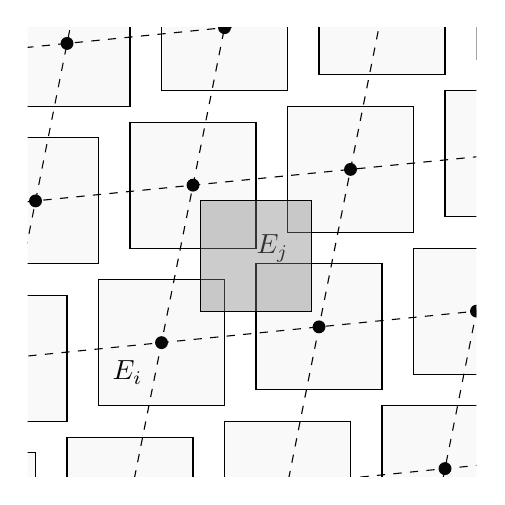
\begin{tikzpicture}
			%copied from www.texample.net/tikz/examples/lattice-points/ and suitably modified
			
			
			\clip (-1.7,-1.7) rectangle (4cm,4cm); % Clips the picture...
			
			\def\l{2};
			\def\s{0.4};
			\def\S{0.35};
			
			\def\A{1}
			\def\B{0.1}
			\def\C{0.2}
			\def\D{1}
			\begin{scope}
			\pgftransformcm{\A}{\B}{\C}{\D}{\pgfpoint{0cm}{0cm}}
			% This is actually the transformation matrix entries that
			% gives the slanted unit vectors.
			
			\draw[dashed] (-4,-4) grid[step=\l cm] (7,7);
			% Draws a grid in the new coordinates.
			
			\foreach \x in {-4,-3,...,3}{% Two indices running over each
				\foreach \y in {-4,-3,...,3}{% node on the grid we have drawn 
					\node[draw,circle,inner sep=1.5pt,fill] at (\l*\x,\l*\y) {};
					% Places a dot at those points
				}
			}
			
			\node at (-0.1,-0.1) [below left] {$E_i$};
			
			\node at (0.5*\l-0.08,0.5*\l-0.19) [above right] {$E_j$};
			
			
			%\node at (0.5*\l,0.5*\l) {$D$};
			\end{scope}
			
			
			\foreach \x in {-1,-2,0,1,2}{% Two indices running over each
				\foreach \y in {-1,-2,0,1,2}{% node on the grid we have drawn 
					\filldraw[fill=gray, fill opacity=0.05, draw=black] (-\s*\l+\x*\l*\A+\y*\l*\C,-\s*\l+\x*\l*\B+\y*\l*\D)
					rectangle (\s*\l+\x*\l*\A+\y*\l*\C,\s*\l+\x*\l*\B+\y*\l*\D);
					
				}
			}
			
			\filldraw[fill=gray, fill opacity=0.4, draw=black] ({-\S*\l+0.5*\l*(\A+\C)},{-\S*\l+0.5*\l*(\B+\D)})
			rectangle ({\S*\l+0.5*\l*(\A+\C)},{\S*\l+0.5*\l*(\B+\D)});
			
			\end{tikzpicture}
		
		% or use \input{mytikz}
		\caption{Given two charts $E_i$ and $E_j$, the chart $E_j$ is glued to $E_i$ along intersections with all translates of $E_i$ by $q\in M$.}
		\label{glue-cover-tikzpicture}
	\end{figure}
	
	\end{lemma} 
	\begin{proof}
	Since $\mathbb R^r/\Lambda$ is compact, we can find finitely many $s_1,\dots,s_k$ and $d_1,\dots,d_k \in \mathbb{R}^r_{>0}$ such that $\mathbb R^r/\Lambda$ is covered by the $s_i+S(d_i)$. When we choose corresponding $c_1,\dots,c_k \in T(K)$ and $q_1,\dots,q_k$ as in Lemma~\ref{cube around point gives local chart for E/M}, then the corresponding $E_i:=E(c_i,q_i)$ give an admissible cover of $A=E/M$ by admissible open subsets of $E$.
	
	In order to reconstruct $A$, note that $\cup_{m\in M} m\cdot E_i$ is precisely the preimage of $E_i$ under the projection $E\rightarrow E/M$. In particular, the subspace $E_{ij}$ is precisely the preimage of $E_i$ under the composition $E_j\hookrightarrow E \rightarrow E/M$. In other words, the subspace $E_{ij}\subseteq E_j$ is the intersection of $E_i$ and $E_j$ when considered as subspaces of $A$. This shows that as charts of $A$, the spaces $E_i$ and $E_j$ are glued via $E_{ij}$ as described.
	\end{proof}
	Finally, we need some control about what happens to the cubes under $[p]$-multiplication. Recall from Lemma~\ref{cube around point gives local chart for E/M} that we can always assume that $c$ admits $p$-th roots.
	\begin{lemma}\label{pullback of cuboid is cuboid}
		Let $c^{1/p}$ be a $p$-th root of $c$ and let $q^{1/p}$ be a $p$-th root of $q$ in $(K^\times)^r$. Then under $[p]:E\rightarrow E$, the admissible open $E(c_i,q)$ pulls back to the admissible open $E(c_i^{1/p},q^{1/p})$.
	\end{lemma}
	\begin{proof}
		It is clear that under $[p]:T\rightarrow T$, the admissible open cuboid $c\cdot \mathcal B(q,q^{-1})$ centered at $c$ pulls back to $c^{1/p}\cdot \mathcal B(q^{1/p},q^{-1/p})$. Note that this is independent of the choices of $c^{1/p}$ and $q^{1/p}$. Now recall that in terms of fibre bundles, multiplication $[p]:E\rightarrow E$ is
		\[[p]\times^{[p]}[p]: T\times^{\overline{T}_\eta}\overline{E}_\eta\rightarrow T\times^{\overline{T}_\eta}\overline{E}_\eta \]
		by Lemma~\ref{p-multiplication is induced from Borel construction}. Thus $(c\cdot \mathcal B(q,q^{-1}))\times^{\overline{T}_\eta}\overline{E}_\eta$ pulls back to $(c^{1/p}\cdot \mathcal B(q^{1/p},q^{-1/p}))\times^{\overline{T}_\eta}\overline{E_\eta}$.
	\end{proof}

	\subsection{The two towers}
	In this section we want to separate the $[p]$-multiplication of $A$ into two different towers, which we think of as being a ``ramified'' tower and an ``\'etale'' tower. Of course in characteristic $0$ both towers will actually be \'etale, and these words are only meant to describe the behaviour of the maps relative to the lattice $M$.
	
	For the ramified tower, we first make an auxiliary choice of certain torsion subgroups of $A$: Since $K$ is algebraically closed, we can choose lattices $M^{1/p^n}\subseteq E$ such that $[p]:E\rightarrow E$ restricts to isomorphisms $M^{1/p^{n+1}}\rightarrow M^{1/p^n}$ for all $n$.
	
	\begin{remark}\label{remark: Definition of the D_n}
		Such a choice is equivalent to the choice of subgroups $D_n\subseteq A[p^n]$ of rank $p^{rn}$ for all $n$ such that $pD_{n+1}=D_n$ and $D_n+E[p^n]=A[p^n]$. Namely,
		given the lattices $M^{1/p^{n+1}}$, we obtain the desired torsion subgroups by setting $D_n:=M^{1/p^{n+1}}/M$. This is because any such lattice gives a splitting of the short exact sequence $0\rightarrow E[p^n]\rightarrow A[p^n]\rightarrow M/M^{p^n} \rightarrow 0$.
		
		Conversely, given subgroups $D_n\subseteq A[p^n]$ with properties as above, we recover $M^{1/p^n}$ as the kernel of $E\rightarrow A\rightarrow A/D_n$.
		
		One might call the choice of $D_n$ for all $n$ a partial anticanonical $\Gamma_0(p^\infty)$-structure, because if $B$ admits a canonical subgroup (that is, if $B$ has bad reduction or if it has good reduction and the reduction satisfies a condition on its Hasse invariant), the choice of a (full) anticanonical $\Gamma_0(p^\infty)$-structure on $A$ is equivalent to the choice of a partial anticanonical $\Gamma_0(p^\infty)$-structure on $A$ and an anticanonical $\Gamma_0(p^\infty)$-structure on $B$. Note however that $A$ always has a partial anticanonical subgroup even if $B$ does not have a canonical subgroup.
		
		Note that in the case of $K$ perfectoid but not necessarily algebraically closed, one can still carry out the constructions in the following using partial anticanonical $\Gamma_0(p^\infty)$-structures, whereas the lattices $M^{1/p^n}$ might not be defined over $K$.
	\end{remark}
	
	Following the remark, denote by $D_n$ the torsion subgroup $M^{1/p^n}/M\subseteq A$. The quotient $A/D_n = E/M^{1/p^n}$ is then another abeloid variety over $K$ and the quotient map $v^n:E/M\rightarrow E/M^{1/p^n}$ is an isogeny of degree $p^{rn}$  through which  $[p^n]:A\rightarrow A$ factors: 
		\begin{center}
			\begin{equation}\label{factorisation of [p] over E/M}
			\begin{tikzcd}
				& E/M^{1/p^n} \arrow[rd, "{[p^n]}"] &  \\
				E/M \arrow[rr, "{[p^n]}"] \arrow[ru,"v^n"] &  & E/M.
			\end{tikzcd}
			\end{equation}
		\end{center}
		We think of these maps as being an analogue of Frobenius and Verschiebung, which is why we denote the left map by $v$.
		Putting everything together, the $[p]$-multiplication tower splits into two towers
		\begin{center}
		\begin{equation}\label{p-multiplication tower of E/M splits into vertical and horizontal tower}
		\begin{tikzcd}[column sep={1.1cm,between origins},row sep={0.7cm,between origins}]
			\ddots \arrow[rd] &  &  & \vdots \arrow[d] &  & \vdots \arrow[d] \\
			& E/M \arrow[rr,"v"] \arrow[rrdd, "{[p]}"'] &  & E/M^{1/p} \arrow[rr,"v"] \arrow[dd,"{[p]}"] &  & E/M^{1/p^2} \arrow[dd,"{[p]}"] \\
			&  &  &  &  &  \\
			&  &  & E/M \arrow[rrdd, "{[p]}"'] \arrow[rr,"v"] &  & E/M^{1/p} \arrow[dd,"{[p]}"] \\
			&  &  &  &  &  \\.
			&  &  &  &  & E/M
		\end{tikzcd}
		\end{equation}
		\end{center}
		Since each quotient $M^{1/p^n}/M$ is a finite \'etale group scheme, all horizontal maps are finite \'etale. The vertical tower on the other hand fits into a second commutative diagram of rigid groups which compares it to the $[p]$-tower of $E$:
		
		\begin{center}
		\begin{equation}\label{F-tower for E/M}
		\begin{tikzcd}
			& \vdots \arrow[d] & \vdots \arrow[d] & \vdots \arrow[d] &  \\
			0 \arrow[r] & M^{1/p^2} \arrow[d, "\cong"] \arrow[r] & E \arrow[d, "{[p]}"] \arrow[r] & E/M^{1/p^2} \arrow[d, "{[p]}"] \arrow[r] & 0 \\
			0 \arrow[r] & M^{1/p} \arrow[d, "\cong"] \arrow[r] & E \arrow[d, "{[p]}"] \arrow[r] & E/M^{1/p} \arrow[d, "{[p]}"] \arrow[r] & 0 \\
			0 \arrow[r] & M \arrow[r] & E \arrow[r] & E/M \arrow[r] & 0
		\end{tikzcd}
		\end{equation}
		\end{center}
		
		\subsection{Constructing a limit of the vertical tower}
		
		Our first step is to show that the tower on the right has a perfectoid tilde-limit.
		Recall from Lemma~\ref{an admissible cover of A by cuboids of E} that $E/M$ can be covered by admissible open subspaces $E_1,\dots,E_k\subseteq E$ which map isomorphically onto an admissible open via $E\to E/M$. Denote by $E_i^{1/p^n}\subseteq E$ the pullback along $[p^n]:E\rightarrow E$. Also denote by $E_{ij}^{1/p^n}\subseteq E$ the pullback of the intersection $E_{ij}$. We can then reconstruct the space $E/M^{1/p^n}$ from the $E_i^{1/p^n}$ as follows:
		\begin{lemma}\label{compatible cuboid charts for the tower over E/M}
			\leavevmode
			\begin{enumerate}
		\item The restriction to $E_{i}^{1/p^n}\subseteq E$ of $E\rightarrow E/M^{1/p^n}$ is an isomorphism onto its image. In particular, we can view $E_{i}^{1/p^n}$ as a chart of $E/M^{1/p^n}$, and this is the preimage of $E_i$ under $E/M^{1/p^n}\rightarrow E/M$.
		\item The collection of  $E_{i}^{1/p^n}$ is an atlas for  $E/M^{1/p^n}$. 
		\item We can reconstruct $E/M^{1/p^n}$ from glueing the $E_{i}^{1/p^n}$ along the $E_{ij}^{1/p^n}$.
		\item The map $[p^n]:E/M^{1/p^n}\rightarrow E/M$ can be glued from the restrictions of $[p^n]:E\rightarrow E$ to $E_{i}^{1/p^n}\rightarrow E_{i}$, that is these maps commute with the glueing maps on $E_{ij}^{1/p^n}$.
		\end{enumerate}
		The situation is thus like in Figure~\ref{transform-glue-cover-tikzpicture}.
		\end{lemma}
			\begin{figure}
				
				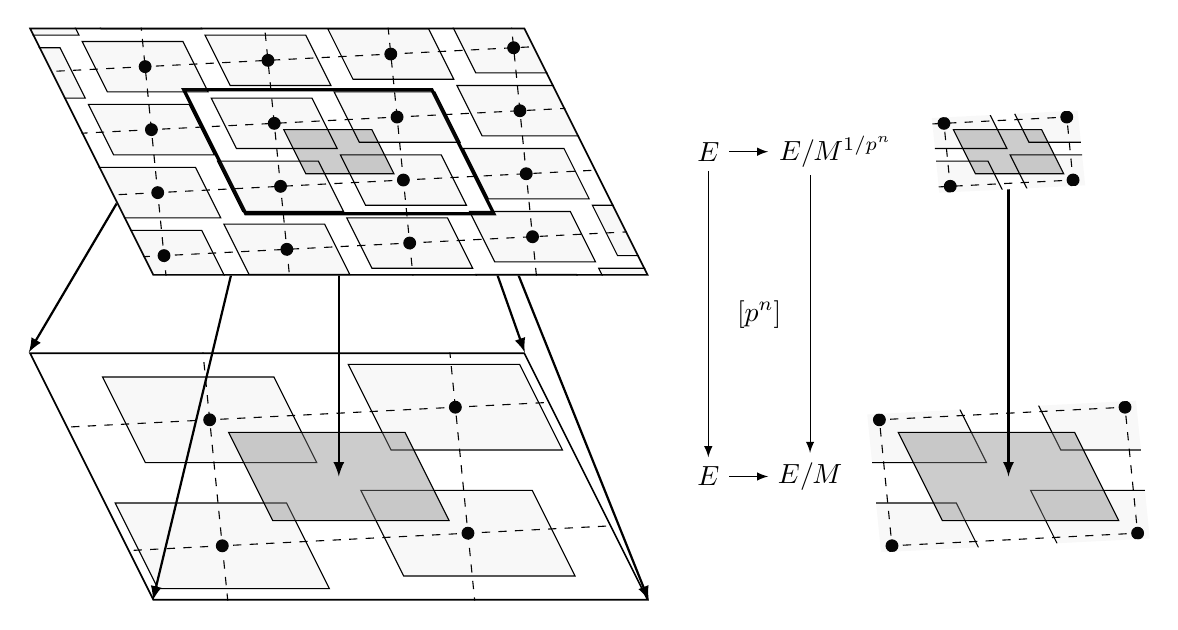
\begin{tikzpicture}
				
				
				0.75
				
				\def\shift{5.5*0.75}
				
				\def\Aoffset{0.15}
				
				%\pgfmathsetmacro\l{2.3*0.75}
				%\pgfmathsetmacro\L{3.5*0.75}
				%\def\s{0.4}
				%\def\S{0.35}
				%\def\Cl{4.55*0.75}
				
				
				\pgfmathsetmacro\l{2*0.8}
				\pgfmathsetmacro\L{4*0.8}
				\def\s{0.34}
				\def\S{0.35}
				\def\Cl{4.2*0.75}
				
				\pgfmathsetmacro\hoffset{\Cl/(4.55*0.75)*1.4}
				
				\def\hshift{2.7*\Cl}
				
				\def\A{1}
				\def\B{0.1}
				\def\C{0.2}
				\def\D{1}
				\pgfmathsetmacro\det{1/(\A*\D-\B*\C)}
				
				\def\AA{1}
				\def\CC{0}
				\def\BB{-0.25}
				\def\DD{0.5}
				
				\begin{scope}
				
				\pgftransformcm{\AA}{\CC}{\BB}{\DD}{\pgfpoint{0cm}{0cm}}
				
				\clip (-\Cl,-\Cl) rectangle (\Cl cm,\Cl cm); % Clips the picture...
				
				\filldraw[very thick,fill=white, fill opacity=1, draw=black] (-\Cl,-\Cl)
				rectangle (\Cl,\Cl);	
				
				\begin{scope}
				\pgftransformcm{\A}{\B}{\C}{\D}{\pgfpoint{0cm}{0cm}}
				% This is actually the transformation matrix entries that
				% gives the slanted unit vectors.
				\draw[dashed] (-2*\Cl,-2*\Cl) grid[step=\L cm,xshift=0.5*\L cm,yshift=0.5*\L cm] (3*\Cl,3*\Cl);
				% Draws a grid in the new coordinates.
				
				\foreach \x in {-4.5,-3.5,...,3.5}{% Two indices running over each
					\foreach \y in {-4.5,-3.5,...,3.5}{% node on the grid we have drawn 
						\node[draw,circle,inner sep=1.5pt,fill] at (\L*\x,\L*\y) {};
						% Places a dot at those points
					}
				}
				
				\end{scope}
				
				\foreach \x in {-4.5,-3.5,...,3.5}{% Two indices running over each
					\foreach \y in {-4.5,-3.5,...,3.5}{% node on the grid we have drawn 
						\filldraw[fill=gray, fill opacity=0.05, draw=black] (-\s*\L+\x*\L*\A+\y*\L*\C,-\s*\L+\x*\L*\B+\y*\L*\D)
						rectangle (\s*\L+\x*\L*\A+\y*\L*\C,\s*\L+\x*\L*\B+\y*\L*\D);
						
					}
				}
				
				\filldraw[fill=gray, fill opacity=0.4, draw=black] ({-\S*\L},{-\S*\L})
				rectangle ({\S*\L},{\S*\L});
				
				\end{scope}
				
				
				
				
				\begin{scope}[shift = {(\hshift,0)}]
				\pgftransformcm{\AA}{\CC}{\BB}{\DD}{\pgfpoint{0cm}{0cm}}
				
				
				\pgftransformcm{\A}{\B}{\C}{\D}{\pgfpoint{0cm}{0cm}}
				\clip (-0.5*\L-\Aoffset,-0.5*\L-\Aoffset) rectangle (0.5*\L+\Aoffset,0.5*\L+\Aoffset); % Clips the picture...
				\pgftransformcm{\det*\D}{-\det*\B}{-\det*\C}{\det*\A}{\pgfpoint{0cm}{0cm}}
				
				\filldraw[very thick,fill=white, fill opacity=1, draw=black] (-\Cl,-\Cl)
				rectangle (\Cl,\Cl);	
				
				\begin{scope}
				\pgftransformcm{\A}{\B}{\C}{\D}{\pgfpoint{0cm}{0cm}}
				% This is actually the transformation matrix entries that
				% gives the slanted unit vectors.
				\draw[dashed] (-2*\Cl,-2*\Cl) grid[step=\L cm,xshift=0.5*\L cm,yshift=0.5*\L cm] (3*\Cl,3*\Cl);
				% Draws a grid in the new coordinates.
				
				\foreach \x in {-4.5,-3.5,...,3.5}{% Two indices running over each
					\foreach \y in {-4.5,-3.5,...,3.5}{% node on the grid we have drawn 
						\node[draw,circle,inner sep=1.5pt,fill] at (\L*\x,\L*\y) {};
						% Places a dot at those points
					}
				}
				
				\end{scope}
				
				\foreach \x in {-4.5,-3.5,...,3.5}{% Two indices running over each
					\foreach \y in {-4.5,-3.5,...,3.5}{% node on the grid we have drawn 
						\filldraw[fill=gray, fill opacity=0.05, draw=black] (-\s*\L+\x*\L*\A+\y*\L*\C,-\s*\L+\x*\L*\B+\y*\L*\D)
						rectangle (\s*\L+\x*\L*\A+\y*\L*\C,\s*\L+\x*\L*\B+\y*\L*\D);
						
					}
				}
				
				\filldraw[fill=gray, fill opacity=0.4, draw=black] ({-\S*\L},{-\S*\L})
				rectangle ({\S*\L},{\S*\L});
				
				\pgftransformcm{\A}{\B}{\C}{\D}{\pgfpoint{0cm}{0cm}}{
					\clip (-\l,-\l) rectangle (\l,\l);}
				\end{scope}
				
				
				
				
				
				\pgfmathsetmacro\cl{\Cl*\l/\L} ;
				\draw [thick,-latex] ({-\cl*(\AA+\BB)},{\shift-\cl*(\CC+\DD)}) -- ({-\Cl*(\AA+\BB)},{-\Cl*(\CC+\DD)});
				\draw [thick,-latex] ({-\cl*\BB+\cl*\AA)},{\shift-\cl*(\CC+\DD)}) --({-\Cl*\BB+\Cl*\AA)},{\Cl*\CC-\Cl*\DD)});
				\draw [thick,-latex] ({\cl*\BB+\cl*\AA)},{\shift+\cl*(\CC+\DD)}) --({\Cl*\BB+\Cl*\AA)},{\Cl*\CC+\Cl*\DD)});
				\draw [thick,-latex] ({\cl*\BB-\cl*\AA)},{\shift+\cl*(\CC+\DD)}) --({\Cl*\BB-\Cl*\AA)},{-\Cl*\CC+\Cl*\DD)});
				
				
				\draw [thick,-latex] (0,\shift) --(0,0);
				\draw [thick,-latex] (\hshift,\shift) --(\hshift,0);
				
				\def\A{1}
				\def\B{0.1}
				\def\C{0.2}
				\def\D{1}
				
				
				
				
				
				\begin{scope}[shift={(0,\shift)}]
				\pgftransformcm{\AA}{\CC}{\BB}{\DD}{\pgfpoint{0cm}{0cm}}
				\coordinate (Origin)   at (0,0);
				\coordinate (XAxisMin) at (-2,0);
				\coordinate (XAxisMax) at (3.7,0);
				\coordinate (YAxisMin) at (0,-2);
				\coordinate (YAxisMax) at (0,3.7);
				
				
				\coordinate (offset)   at ({0.5*\l*(\A+\C)},{0.5*\l*(\B+\D)});
				
				
				\clip (-\Cl,-\Cl) rectangle (\Cl cm,\Cl cm); % Clips the picture...
				
				
				\filldraw[very thick,fill=white, fill opacity=1, draw=black] (-\Cl,-\Cl) 
				rectangle (\Cl,\Cl);
				\filldraw[very thick,fill=white, fill opacity=0.1, draw=black] (-\Cl*\l/\L,-\Cl*\l/\L) 
				rectangle (\Cl*\l/\L,\Cl*\l/\L);
				
				
				
				\filldraw[fill=gray, fill opacity=0.4, draw=black] ({-\S*\l},{-\S*\l})
				rectangle ({\S*\l},{\S*\l});
				
				\def\s{0.4};
				\def\S{0.35};
				
				\begin{scope}
				\pgftransformcm{\A}{\B}{\C}{\D}{\pgfpoint{0cm}{0cm}}
				% This is actually the transformation matrix entries that
				% gives the slanted unit vectors.
				
				\draw[dashed] (-2*\Cl,-2*\Cl) grid[step=\l cm,xshift=0.5*\l cm,yshift=0.5*\l cm] (7,7);
				% Draws a grid in the new coordinates.
				
				\foreach \x in {-4.5,-3.5,...,3.5}{% Two indices running over each
					\foreach \y in {-4.5,-3.5,...,3.5}{% node on the grid we have drawn 
						\node[draw,circle,inner sep=1.5pt,fill] at (\l*\x,\l*\y) {};
						% Places a dot at those points
					}
				}
				
				
				%\node at (0.5*\l,0.5*\l) {$D$};
				\end{scope}
				
				
				\foreach \x in {-4.5,-3.5,...,3.5}{% Two indices running over each
					\foreach \y in {-4.5,-3.5,...,3.5}{% node on the grid we have drawn 
						\filldraw[fill=gray, fill opacity=0.05, draw=black] (-\s*\l+\x*\l*\A+\y*\l*\C,-\s*\l+\x*\l*\B+\y*\l*\D)
						rectangle (\s*\l+\x*\l*\A+\y*\l*\C,\s*\l+\x*\l*\B+\y*\l*\D);
						
					}
				}
				
				
				
				\end{scope}
				
				
				
				
				
				
				\begin{scope}[shift = {(\hshift,\shift)}]
				
				\pgftransformcm{\AA}{\CC}{\BB}{\DD}{\pgfpoint{0cm}{0cm}}
				
				
				\pgftransformcm{\A}{\B}{\C}{\D}{\pgfpoint{0cm}{0cm}}
				\clip (-0.5*\l-\Aoffset,-0.5*\l-\Aoffset) rectangle (0.5*\l+\Aoffset,0.5*\l+\Aoffset);
				\pgftransformcm{\det*\D}{-\det*\B}{-\det*\C}{\det*\A}{\pgfpoint{0cm}{0cm}}
				
				\filldraw[very thick,fill=white, fill opacity=1, draw=black] (-\Cl,-\Cl) 
				rectangle (\Cl,\Cl);
				\filldraw[very thick,fill=white, fill opacity=0.1, draw=black] (-\Cl*\l/\L,-\Cl*\l/\L) 
				rectangle (\Cl*\l/\L,\Cl*\l/\L);
				
				
				
				\filldraw[fill=gray, fill opacity=0.4, draw=black] ({-\S*\l},{-\S*\l})
				rectangle ({\S*\l},{\S*\l});
				
				\def\s{0.4};
				\def\S{0.35};
				
				\begin{scope}
				\pgftransformcm{\A}{\B}{\C}{\D}{\pgfpoint{0cm}{0cm}}
				% This is actually the transformation matrix entries that
				% gives the slanted unit vectors.
				
				\draw[dashed] (-2*\Cl,-2*\Cl) grid[step=\l cm,xshift=0.5*\l cm,yshift=0.5*\l cm] (7,7);
				% Draws a grid in the new coordinates.
				
				\foreach \x in {-4.5,-3.5,...,3.5}{% Two indices running over each
					\foreach \y in {-4.5,-3.5,...,3.5}{% node on the grid we have drawn 
						\node[draw,circle,inner sep=1.5pt,fill] at (\l*\x,\l*\y) {};
						% Places a dot at those points
					}
				}
				
				
				%\node at (0.5*\l,0.5*\l) {$D$};
				\end{scope}
				
				
				\foreach \x in {-4.5,-3.5,...,3.5}{% Two indices running over each
					\foreach \y in {-4.5,-3.5,...,3.5}{% node on the grid we have drawn 
						\filldraw[fill=gray, fill opacity=0.05, draw=black] (-\s*\l+\x*\l*\A+\y*\l*\C,-\s*\l+\x*\l*\B+\y*\l*\D)
						rectangle (\s*\l+\x*\l*\A+\y*\l*\C,\s*\l+\x*\l*\B+\y*\l*\D);
						
					}
				}
				
				
				
				\end{scope}
				
				
				\node(Q) at ({\Cl*1.9-\hoffset},\shift) {$E$};
				\node(QQQ)  [label={[label distance=-1.05cm]0:$E/M^{1/p^n}$}] at ({\Cl*1.9},\shift) {\phantom{$E/M$}};
				
				\node(P) at ({\Cl*1.9-\hoffset},0) {$E$};
				\node(PPP) at (({\Cl*1.9},0) {$E/M$};
				
				\node at (({\Cl*1.9-0.5*\hoffset},0.5*\shift) {$[p^n]$};
				
				\draw[-latex] (Q.south) -- (P.north);
				\draw[-latex] (QQQ.south) -- (PPP.north);
				\draw[-latex] (Q.east) -- (QQQ.west);
				\draw[-latex] (P.east) -- (PPP.west);
				
				%\node(Q) at ({\Cl*2.1-\hoffset},\shift) {$E$};
				%\node(QQ) at (({\Cl*2.1},\shift) {$E_j^{1/p^n}$};
				%\node(QQQ)  [label={[label distance=-1.05cm]0:$E/M^{1/p^n}$}] at ({\Cl*2.1+\hoffset},\shift) {\phantom{$E/M$}};
				
				%\node(P) at ({\Cl*2.1-\hoffset},0) {$E$};
				%\node(PP) at (({\Cl*2.1},0) {$E_j$};
				%\node(PPP) at (({\Cl*2.1+\hoffset},0) {$E/M$};
				
				%\draw[-latex] (QQ.south) -- (PP.north);
				%\draw[left hook-latex] (PP.west) -- (P.east);
				%\draw[left hook-latex] (QQ.west) -- (Q.east);
				%\draw[right hook-latex] (QQ.east) -- (QQQ.west);
				%\draw[right hook-latex] (PP.east) -- (PPP.west);
				%\draw[-latex] (Q.south) -- (P.north) node[midway,right] {$[p^n]$};
				%\draw[-latex] (QQQ.south) -- (PPP.north) node[midway,left] {$[p^n]$};
				%
				
				\end{tikzpicture}
				
				\caption{Illustration of how $[p^n]:E/M^{1/p^n}\rightarrow E/M$ can be glued from the maps $E_j^{1/p^n}\rightarrow E_j$. Here $E_j$ on bottom and $E_j^{1/p^n}$ on top are represented by the grey cuboids in the middle. On the left they are embedded into $E$ whereas on the right they are considered as charts for $E/M$ and $E/M^{1/p}$.}
				\label{transform-glue-cover-tikzpicture}
			\end{figure}
		\begin{proof}
		The first part follows because the map on the left of diagram~\ref{F-tower for E/M} is an isomorphism. The second follows from the pullback of the $E_i$ along $E/M^{1/p^n}\rightarrow E/M$, using that the diagram commutes.
		We thus obtain an admissible cover by cuboids $E_1^{1/p^n},\dots,E_k^{1/p^n}$ of $E/M^{1/p^n}$.
		The second part of Lemma~\ref{an admissible cover of A by cuboids of E} applied to $E/M^{1/p^n}$ then shows that $E/M^{1/p^n}$ can be reconstructed by glueing along subspaces $E_{ij}^{1/p^n}$.
		
		Finally, in order to see that one can glue together the map $[p^n]:E/M^{1/p^n}\rightarrow E/M$ from the $E_i^{1/p^n}$, use that intersection of cuboids are again cuboids, and so $E_{ij}^{1/p^n}$ is a disjoint union of cuboids. It then follows from Lemma~\ref{pullback of cuboid is cuboid} that $E_{ij}$ pulls back under $[p^n]$ to the intersection $E_{ij}^{1/p^n}\subseteq E/M^{1/p^n}$. That $[p^n]$ commutes with the glueing maps is clear because we know from diagram (\ref{factorisation of [p] over E/M}) that $[p^n]:E\rightarrow E$ induces a morphism $[p^n]:E/M^{1/p^n}\rightarrow E/M$.
		\end{proof}
		We are now ready to prove:
		\begin{proposition}\label{explicit construction of vertical tilde-limit}
			There is a perfectoid space $E/M^{1/p^\infty}$ such that\[E/M^{1/p^\infty}\sim \varprojlim_{n}E/M^{1/p^n}. \]
		\end{proposition}
		\begin{proof}
		 Denote by $E_i^{1/p^\infty}$ the pullback of $E_i\subseteq E$ to $E_\infty$. This is an open subspace of a perfectoid space and hence perfectoid. Moreover, by Proposition~\ref{SW Proposition 2.4.3} we have  \[ E_i^{1/p^\infty}\sim \varprojlim E_i^{1/p^n}.\] 
		Given two different $E_i$, $E_j$, we know by Lemma~\ref{compatible cuboid charts for the tower over E/M} that at every step in the tower, the pullbacks $E_i^{1/p^n}$ and $E_j^{1/p^n}$ to $E/M^{1/p^n}$ intersect in  $E_{ij}^{1/p^n}$.
		We can thus glue the $E_i^{1/p^\infty}$ along pullbacks $E_{ij}^{1/p^\infty}$ of the intersections $E_{ij}=E_i\cap E_j$ to $E_\infty$ and thus obtain a perfectoid space $E/M^{1/p^\infty}$. This is a tilde-limit for $\varprojlim_{[p]}E/M^{1/p^n}$ because by construction it is so locally, and the definition of tilde-limits in Definition 2.4.1 of \cite{SW} is local on the source.
		\end{proof}
	 
	\subsection{Constructing a limit of the horizontal tower}
	In order to construct a tilde-limit for $\varprojlim A$, we can now use that the horizontal maps in diagram~(\ref{p-multiplication tower of E/M splits into vertical and horizontal tower}) are all finite \'etale. They are even finite covering maps, in the following sense:
	\begin{lemma}\label{horizontal map is covering map}
		For any $0\leq m\leq n$, the preimage of $E_i^{1/p^n}$ from Lemma~\ref{compatible cuboid charts for the tower over E/M} under the horizontal map $v^{n-m}:E/M^{1/p^{m}}\rightarrow E/M^{1/p^n}$ is isomorphic to $p^{r(n-m)}$ disjoint copies of $E_i^{1/p^n}$. More canonically, it can be described as the isomorphic image of $M^{1/p^n}/M^{1/p^m}\times E_i^{1/p^m}$ under the multiplication map $E/M^{1/p^m}\times E/M^{1/p^m}\rightarrow E/M^{1/p^m}$.
	\end{lemma}
	\begin{proof}
		By the first part of Lemma~\ref{compatible cuboid charts for the tower over E/M}, we know that the preimage of $E_i^{1/p^n}$ under the projection $E\rightarrow E/M^{1/p^n}$ is a disjoint union of translates of $E_i^{1/p^n}$ by $M^{1/p^{n}}$. The result then follows because $M^{1/p^{n}}/M^{1/p^{m}} =  \underline{(\mathbb Z/p^{n-m}\mathbb Z)^r}$.
	\end{proof}
	We also record the following immediate consequence:
	
	\begin{lemma}\label{preimage of E_i under p^n is disjoint copies}
		The preimage of $E_i$ under $[p^n]:A\rightarrow A$ is isomorphic to $p^{rn}$ disjoint copies of $E_i^{1/p^n}$. More canonically, we can describe the preimage as the isomorphic image of  $D_n \times E_i^{1/p^n}$ under the multiplication $A\times A\rightarrow A$. The situation is thus as in figure~\ref{local-glueing-[p]-tikzpicture}.
	\end{lemma}
	\begin{figure}
		
		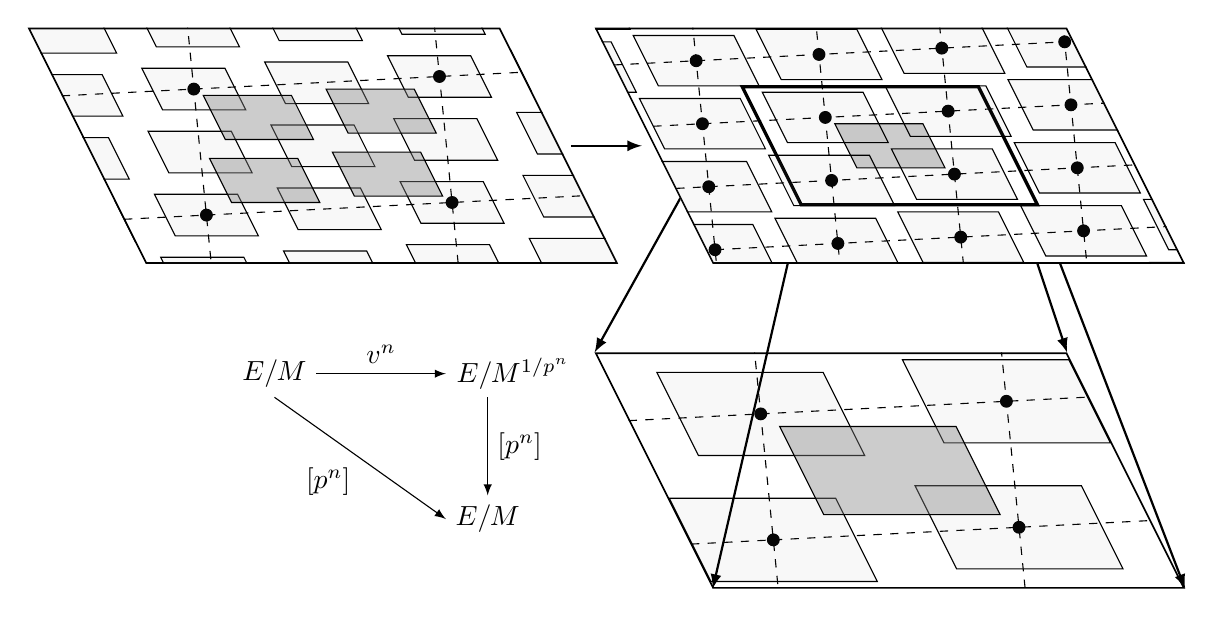
\begin{tikzpicture}
		
		
		\def\shift{5.5*0.75}
		
		\def\Aoffset{0.15}
		\pgfmathsetmacro\l{2*0.8}
		\pgfmathsetmacro\L{4*0.8}
		
		\def\s{0.33}
		\def\S{0.35}
		
		\def\Cl{4*0.75}
		
		\pgfmathsetmacro\hoffset{\Cl/(4.55*0.75)*1.4}
		
		\def\hshift{2.4*\Cl}
		
		\def\A{1}
		\def\B{0.1}
		\def\C{0.2}
		\def\D{1}
		\pgfmathsetmacro\det{1/(\A*\D-\B*\C)}
		
		\def\AA{1}
		\def\CC{0}
		\def\BB{-0.25}
		\def\DD{0.5}
		
		\begin{scope}
		
		\pgftransformcm{\AA}{\CC}{\BB}{\DD}{\pgfpoint{0cm}{0cm}}
		
		\clip (-\Cl,-\Cl) rectangle (\Cl cm,\Cl cm); % Clips the picture...
		
		\filldraw[very thick,fill=white, fill opacity=1, draw=black] (-\Cl,-\Cl)
		rectangle (\Cl,\Cl);	
		
		\begin{scope}
		\pgftransformcm{\A}{\B}{\C}{\D}{\pgfpoint{0cm}{0cm}}
		% This is actually the transformation matrix entries that
		% gives the slanted unit vectors.
		\draw[dashed] (-2*\Cl,-2*\Cl) grid[step=\L cm,xshift=0.5*\L cm,yshift=0.5*\L cm] (3*\Cl,3*\Cl);
		% Draws a grid in the new coordinates.
		
		\foreach \x in {-4.5,-3.5,...,3.5}{% Two indices running over each
			\foreach \y in {-4.5,-3.5,...,3.5}{% node on the grid we have drawn 
				\node[draw,circle,inner sep=1.5pt,fill] at (\L*\x,\L*\y) {};
				% Places a dot at those points
			}
		}
		
		\end{scope}
		
		\foreach \x in {-4.5,-3.5,...,3.5}{% Two indices running over each
			\foreach \y in {-4.5,-3.5,...,3.5}{% node on the grid we have drawn 
				\filldraw[fill=gray, fill opacity=0.05, draw=black] (-\s*\L+\x*\L*\A+\y*\L*\C,-\s*\L+\x*\L*\B+\y*\L*\D)
				rectangle (\s*\L+\x*\L*\A+\y*\L*\C,\s*\L+\x*\L*\B+\y*\L*\D);
				
			}
		}
		
		\filldraw[fill=gray, fill opacity=0.4, draw=black] ({-\S*\L},{-\S*\L})
		rectangle ({\S*\L},{\S*\L});
		
		\end{scope}
		
		
		
		\pgfmathsetmacro\cl{\Cl*\l/\L} ;
		\draw [thick,-latex] ({-\cl*(\AA+\BB)},{\shift-\cl*(\CC+\DD)}) -- ({-\Cl*(\AA+\BB)},{-\Cl*(\CC+\DD)});
		\draw [thick,-latex] ({-\cl*\BB+\cl*\AA)},{\shift-\cl*(\CC+\DD)}) --({-\Cl*\BB+\Cl*\AA)},{\Cl*\CC-\Cl*\DD)});
		\draw [thick,-latex] ({\cl*\BB+\cl*\AA)},{\shift+\cl*(\CC+\DD)}) --({\Cl*\BB+\Cl*\AA)},{\Cl*\CC+\Cl*\DD)});
		\draw [thick,-latex] ({\cl*\BB-\cl*\AA)},{\shift+\cl*(\CC+\DD)}) --({\Cl*\BB-\Cl*\AA)},{-\Cl*\CC+\Cl*\DD)});
		
		\draw [thick,-latex] (-\hshift+\Cl*1.05,\shift )--(-\Cl*1.05,\shift);
		
		
		\def\A{1}
		\def\B{0.1}
		\def\C{0.2}
		\def\D{1}
		
		
		
		
		\begin{scope}[shift={(0,\shift)}]
		\pgftransformcm{\AA}{\CC}{\BB}{\DD}{\pgfpoint{0cm}{0cm}}
		
		\clip (-\Cl,-\Cl) rectangle (\Cl cm,\Cl cm); % Clips the picture...
		
		
		\filldraw[very thick,fill=white, fill opacity=1, draw=black] (-\Cl,-\Cl) 
		rectangle (\Cl,\Cl);
		\filldraw[very thick,fill=white, fill opacity=0.1, draw=black] (-\Cl*\l/\L,-\Cl*\l/\L) 
		rectangle (\Cl*\l/\L,\Cl*\l/\L);
		
		
		
		\filldraw[fill=gray, fill opacity=0.4, draw=black] ({-\S*\l},{-\S*\l})
		rectangle ({\S*\l},{\S*\l});
		
		\def\s{0.4};
		\def\S{0.35};
		
		\begin{scope}
		\pgftransformcm{\A}{\B}{\C}{\D}{\pgfpoint{0cm}{0cm}}
		% This is actually the transformation matrix entries that
		% gives the slanted unit vectors.
		
		\draw[dashed] (-2*\Cl,-2*\Cl) grid[step=\l cm,xshift=0.5*\l cm,yshift=0.5*\l cm] (7,7);
		% Draws a grid in the new coordinates.
		
		\foreach \x in {-4.5,-3.5,...,3.5}{% Two indices running over each
			\foreach \y in {-4.5,-3.5,...,3.5}{% node on the grid we have drawn 
				\node[draw,circle,inner sep=1.5pt,fill] at (\l*\x,\l*\y) {};
				% Places a dot at those points
			}
		}
		
		
		%\node at (0.5*\l,0.5*\l) {$D$};
		\end{scope}
		
		
		\foreach \x in {-4.5,-3.5,...,3.5}{% Two indices running over each
			\foreach \y in {-4.5,-3.5,...,3.5}{% node on the grid we have drawn 
				\filldraw[fill=gray, fill opacity=0.05, draw=black] (-\s*\l+\x*\l*\A+\y*\l*\C,-\s*\l+\x*\l*\B+\y*\l*\D)
				rectangle (\s*\l+\x*\l*\A+\y*\l*\C,\s*\l+\x*\l*\B+\y*\l*\D);
				
			}
		}
		
		\end{scope}
		
		\begin{scope}[shift={(-\hshift,\shift)}]
		\pgftransformcm{\AA}{\CC}{\BB}{\DD}{\pgfpoint{0cm}{0cm}}
		
		
		\clip (-\Cl,-\Cl) rectangle (\Cl cm,\Cl cm); % Clips the picture...
		
		
		\filldraw[very thick,fill=white, fill opacity=1, draw=black] (-\Cl,-\Cl) 
		rectangle (\Cl,\Cl);
		%\filldraw[very thick,fill=white, fill opacity=0.1, draw=black] (-\Cl*\l/\L,-\Cl*\l/\L) 
		%rectangle (\Cl*\l/\L,\Cl*\l/\L);
		
		
		\begin{scope}
		\pgftransformcm{\A}{\B}{\C}{\D}{\pgfpoint{0cm}{0cm}}
		% This is actually the transformation matrix entries that
		% gives the slanted unit vectors.
		
		\draw[dashed] (-2*\Cl,-2*\Cl) grid[step=\L cm,xshift=0.5*\L cm,yshift=0.5*\L cm] (7,7);
		% Draws a grid in the new coordinates.
		
		\foreach \x in {-4.5,-3.5,...,3.5}{% Two indices running over each
			\foreach \y in {-4.5,-3.5,...,3.5}{% node on the grid we have drawn 
				\node[draw,circle,inner sep=1.5pt,fill] at (\L*\x,\L*\y) {};
				% Places a dot at those points
			}
		}
		
		
		%\node at (0.5*\l,0.5*\l) {$D$};
		\end{scope}
		
		
		\foreach \x in {-4,-3,...,3.5}{% Two indices running over each
			\foreach \y in {-4,-3,...,3.5}{% node on the grid we have drawn 
				\filldraw[fill=gray, fill opacity=0.05, draw=black] (-\s*\l+\x*\l*\A+\y*\l*\C,-\s*\l+\x*\l*\B+\y*\l*\D)
				rectangle (\s*\l+\x*\l*\A+\y*\l*\C,\s*\l+\x*\l*\B+\y*\l*\D);
				
			}
		}
		\foreach \x in {-0.5,0.5}{% Two indices running over each
			\foreach \y in {-0.5,0.5}{% node on the grid we have drawn 
				\filldraw[fill=gray, fill opacity=0.4, draw=black] (-\S*\l+\x*\l*\A+\y*\l*\C,-\S*\l+\x*\l*\B+\y*\l*\D)
				rectangle (\S*\l+\x*\l*\A+\y*\l*\C,\S*\l+\x*\l*\B+\y*\l*\D);
				
			}
		}
		
		
		
		\end{scope}
		
		
		\pgfmathsetmacro\hoffset{\Cl/(4.55*0.75)*1.4}
		
		\node(X) at ({-\hshift-0.5*\hoffset},+\hoffset) {$E/M$};
		\node(Y)  [label={[label distance=-1.05cm]0:$E/M^{1/p^n}$}] at ({-\hshift+1.7*\hoffset},+\hoffset) {\phantom{$E/M$}};
		\node(Z) at ({-\hshift+1.7*\hoffset},-0.5*\hoffset) {$E/M$};
		
		\draw[-latex] (Y.south) -- (Z.north) node[midway,right] {$[p^n]$};
		\draw[-latex] (X.east) -- (Y.west) node[midway,above] {$v^n$};
		\draw[-latex] (X.south) -- (Z.west) node[midway,below left] {$[p^n]$};
		
		%\node(QQ) at (({\Cl*2.1},\shift) {$E_j^{1/p^n}$};
		%\node(QQQ)  [label={[label distance=-1.05cm]0:$E/M^{1/p^n}$}] at ({\Cl*2.1+\hoffset},\shift) {\phantom{$E/M$}};
		
		%\node(P) at ({\Cl*2.1-\hoffset},0) {$E$};
		%\node(PP) at (({\Cl*2.1},0) {$E_j$};
		%\node(PPP) at (({\Cl*2.1+\hoffset},0) {$E/M$};
		
		%\draw[-latex] (QQ.south) -- (PP.north);
		%\draw[left hook-latex] (PP.west) -- (P.east);
		%\draw[left hook-latex] (QQ.west) -- (Q.east);
		%\draw[right hook-latex] (QQ.east) -- (QQQ.west);
		%\draw[right hook-latex] (PP.east) -- (PPP.west);
		%\draw[-latex] (Q.south) -- (P.north) node[midway,right] {$[p^n]$};
		%\draw[-latex] (QQQ.south) -- (PPP.north) node[midway,left] {$[p^n]$};
		%
		
		\end{tikzpicture}
		
		\caption{Illustration of how $[p]:E/M\rightarrow E/M$ factors in a part that is ``ramified'' (the vertical tower) and a part that is ``\'etale'' (the horizontal tower) with respect to our cover.}
		\label{local-glueing-[p]-tikzpicture}
	\end{figure}
	\begin{proof}
		This follows from the first part of Lemma~\ref{compatible cuboid charts for the tower over E/M} combined with Lemma~\ref{horizontal map is covering map} in the case of $m=0$.
	\end{proof}
	
	
	\begin{lemma}\label{squares in double tower are pullbacks}
		The squares in diagram~(\ref{p-multiplication tower of E/M splits into vertical and horizontal tower}) are all pullback diagrams.
		\begin{center}
			\begin{tikzcd}
				E/M^{1/p^n} \arrow[d, "{[p]}"] \arrow[r,"v"] & E/M^{1/p^{n+1}} \arrow[d, "{[p]}"] \\
				E/M^{1/p^{n-1}} \arrow[r,"v"] & E/M^{1/p^n}
			\end{tikzcd}
		\end{center}
	\end{lemma}
	\begin{proof}
		This can for instance be checked locally: The admissible open subset $E_i^{1/p^n}\subseteq E/M^{1/p^n}$ from Lemma~\ref{compatible cuboid charts for the tower over E/M} is pulled back to $E_i^{1/p^{n+1}}$ under the vertical map $[p]:E/M^{1/p^{n+1}}\rightarrow E/M^{1/p^n}$. The preimage of $E_i^{1/p^n}$ under the horizontal map $E/M^{1/p^{n-1}}\rightarrow E/M^{1/p^n}$ is $p^r$ disjoint copies of $E_i^{1/p^n}$ by Lemma~\ref{horizontal map is covering map}. The pullback of $E_i^{1/p^n}$ to the upper right is thus $p^r$ disjoint copies of $E_i^{1/p^{n+1}}$, which is clearly the fibre product.
	\end{proof}
	\begin{lemma}\label{horizontal etale map pulls back to vertical limit}
	The horizontal maps in diagram~(\ref{p-multiplication tower of E/M splits into vertical and horizontal tower}) induce natural finite \'etale morphisms $v:E/M^{1/p^\infty}\rightarrow E/M^{1/p^\infty}$ that fit into Cartesian diagrams
	\begin{center}
		\begin{tikzcd}
			E/M^{1/p^\infty} \arrow[d, "{}"] \arrow[r,"v^m"] & E/M^{1/p^\infty} \arrow[d, "{}"] \\
			E/M^{1/p^{n-m}} \arrow[r,"v^m"] & E/M^{1/p^{n}}
		\end{tikzcd}
	\end{center}
	In particular, the preimage of $E_i^{1/p^\infty}$ under $v^m$ is isomorphic to $p^{rm}$ copies of $E_i^{1/p^\infty}$.
	\end{lemma}
	\begin{proof}
		Since $E/M \rightarrow E/M^{1/p}$ is finite \'etale, the fibre product with $E/M^{1/p^\infty} \rightarrow E/M^{1/p}$ exists and is perfectoid by Proposition~7.10 of \cite{perfectoid}.
		
		The universal property of the fibre product then gives a unique map 
		\[E/M^{1/p^\infty}\rightarrow E/M\times_ {E/M^{1/p}}E/M^{1/p^\infty}\]
		making the natural diagrams commute.
		On the other hand, using Lemma~\ref{squares in double tower are pullbacks} we see that the fibre product has compatible maps into the vertical inverse system over $E/M$. Since by Proposition~\ref{SW Proposition 2.4.5} the perfectoid tilde-limit $E/M^{1/p^\infty}$ is universal for maps from perfectoid spaces to the inverse system, we obtain a unique map into the other direction.
	\end{proof}
	We thus obtain a pro-\'etale tower
	\begin{equation}\label{proetale tower in the vertical limit}
	\dots \xrightarrow{v}E/M^{1/p^\infty}\xrightarrow{v} E/M^{1/p^\infty}\xrightarrow{v} E/M^{1/p^\infty}
	\end{equation}
	which we think of as being a kind of vertical ``limit'' of diagram~\ref{p-multiplication tower of E/M splits into vertical and horizontal tower}. 
	
	We now want to explicitly construct a tilde-limit of this tower. Recall from Remark~\ref{remark: Definition of the D_n} the finite \'etale subgroups $D_n=M^{1/p^n}/M\subseteq E/M=A$. Since $K$ is algebraically closed, they are constant and uncanonically isomorphic to $(\underline{\mathbb Z/p^{n}\mathbb Z})^{r}=\operatorname{Spa}(\operatorname{Map}(\mathbb (\mathbb Z/p^n\mathbb Z)^r,K),\operatorname{Map}((\mathbb Z/p^n\mathbb Z)^r,\mathcal O_K))$.
	The $[p]$-multiplication on $E$ maps $M^{1/p^{n+1}}$ onto $M^{1/p^{n}}$ and therefore the $[p]$-multiplication tower of $E/M$ induces a tower
	\[\dots \xrightarrow{[p]}D_{n+1}\xrightarrow{[p]}D_n\rightarrow\dots.\]
	
	\begin{lemma}There exists a perfectoid space $D_\infty$ such that $D_\infty\sim\varprojlim_{[p]} D_n$. Any choice of compatible isomorphisms $D_n\cong\underline{\mathbb Z/p^{n}\mathbb Z}^{r}$ induces an isomorphism 
		\[D_\infty = \operatorname {Spa}(\operatorname{Map}_{cts}(\mathbb Z_p^{r},K),\operatorname{Map}_{cts}(\mathbb Z_p^{r},\mathcal O_K)).\]
	\end{lemma}
	
	Such "profinite" perfectoid spaces like $D_\infty$ are mentioned in \cite{berkeley} before Remark 8.2.2.
	\begin{proof}
		The $D_n$ are \'etale over $(K,\mathcal O_K)$ and thus affinoid perfectoid. Proposition~\ref{proposition: tilde-limits of perfectoid spaces} then shows that $D_\infty$ exists. Given isomorphisms $D_n=(\underline{\mathbb Z/p^{n}\mathbb Z})^{r}=\operatorname{Spa}(\operatorname{Map}(\mathbb (\mathbb Z/p^n\mathbb Z)^r,K),\operatorname{Map}((\mathbb Z/p^n\mathbb Z)^r,\mathcal O_K))$, Proposition~\ref{proposition: tilde-limits of perfectoid spaces} moreover says that the tilde-limit is given by the $\pi$-adic completion of 
		\[\big(\varinjlim_n \operatorname{Map}((\mathbb Z/p^n\mathbb Z)^r,K),\varinjlim_n \operatorname{Map}((\mathbb Z/p^n\mathbb Z)^r,\mathcal O_K)\big) = (\operatorname{Map}_{lc}(\mathbb Z_p^r,K),\operatorname{Map}_{lc}(\mathbb Z_p^r,\mathcal O_K))\]
		where $\operatorname{Map}_{lc}$ denotes the locally constant morphisms, for the $p$-adic topology on $\mathbb Z_p$. Since the $\pi$-adic completion of these are the continuous morphisms, this proves the Lemma.
	\end{proof}
	
	\begin{proposition}\label{horizontal limit of vertical limit}
	There exists a perfectoid space $(E/M^{1/p^\infty})_\infty$ such that \[(E/M^{1/p^\infty})_\infty\sim \varprojlim_{v}(E/M^{1/p^\infty}).\]
	 Moreover, the projection map $\pi:(E/M^{1/p^\infty})_\infty\rightarrow E/M^{1/p^\infty}$ is a profinite covering map, namely every point of $E/M^{1/p^\infty}$ has an open neighbourhood $U$ such that $\pi^{-1}(U)$ is isomorphic to $D_\infty \times U$.
	\end{proposition}
	\begin{proof}
	By Lemma~\ref{horizontal etale map pulls back to vertical limit}, the preimage of $E_i^{1/p^\infty}$ under $v^m$ of $E/M^{1/p^\infty}$ is isomorphic to $D_m\times E_i^{1/p^\infty}$. By Lemma~\ref{affinoid tilde-limits commute with fibre products} we then have
	\[D_\infty \times E_i^{1/p^\infty}\sim \varprojlim_m D_m\times E_i^{1/p^\infty}.\]
	
	As before, these local tilde-limits glue using Propositions~\ref{SW Proposition 2.4.3} and \ref{SW Proposition 2.4.5}.
	\end{proof}
	
	\subsection{The diagonal tower: proof of the main theorem}
	We now want to show that $(E/M^{1/p^\infty})_\infty$ is in fact a tilde-limit of the $[p]$-multiplication tower. In other words, this says that the horizontal limit of the vertical tilde-limits in diagram~\ref{p-multiplication tower of E/M splits into vertical and horizontal tower} is also a diagonal tilde-limit.
	This isn't just a formal consequence since tilde-limits aren't limits. But using the local geometry of the maps in the tower in terms of cuboids, it is still easy to see:
	
	\begin{proposition}\label{tilde-limit of tilde-limits of partial towers is tilde-limit of whole tower}
		The perfectoid space  $A_\infty:=(E/M^{1/p^\infty})_\infty$ is a tilde-limit of $\varprojlim_{[p]}A$.	It is independent up to unique isomorphism of the choice of partial anticanonical $\Gamma_0(p^\infty)$-structure, but it remembers the choice as a pro-finite \'etale closed subgroup $D_\infty \subseteq A_\infty$. 
		
		The preimage of $E_i\subseteq A$ under the projection $A_\infty \rightarrow A$ is isomorphic to $D_\infty \times E_i^{1/p^\infty}$.
	\end{proposition}
	\begin{proof}
	It is clear from $(E/M^{1/p^\infty})_\infty \sim \varprojlim_v E/M^{1/p^\infty}$ and $E/M^{1/p^\infty}\sim \varprojlim_{[p]} E/M^{1/p^n}$ that the underlying topological space of $(E/M^{1/p^\infty})_\infty$ is indeed isomorphic to $\varprojlim_{[p]}|E/M|$.

	In order to show that it is a tilde-limit of $\varprojlim_{[p]}E/M$, it thus suffices to give an explicit cover of $(E/M^{1/p^\infty})_\infty$ by open affinoids satisfying the tilde-limit property. 
	
	Recall that by construction of $(E/M^{1/p^\infty})$ we have a cover of $E/M$ by open subsets $E_i$ that pull back to perfectoid open subspaces $E_i^{1/p^\infty}$ for which $E_i^{1/p^\infty}\sim \varprojlim E_i^{1/p^n}$.
	 Moreover, by the second part of Proposition~\ref{horizontal limit of vertical limit} we know that the pullback of $E_i^{1/p^\infty}$ to $(E/M^{1/p^\infty})_\infty$ is $D_\infty \times E_i^{1/p^\infty}$. 
	 
	 On the other hand, when we go along the diagonal tower, we obtain the inverse system 
	 \[\dots\rightarrow D_{n+1}\times E_i^{1/p^{n+1}}\rightarrow D_{n}\times E_i^{1/p^{n}}\rightarrow \dots.\]
	 
	By Lemma~\ref{affinoid tilde-limits commute with fibre products} this inverse system has perfectoid tilde-limit $D_\infty \times E_i^{1/p^\infty}$. These local tilde-limits glue together to give the desired tilde-limit $A_\infty$.
	 
	That $A_\infty$ is independent of the $\Gamma_0(p^\infty)$-structure up to unique isomorphism is a consequence of the universal property of the perfectoid tilde-limit. To see that $D_\infty$ is a closed subgroup of $A_\infty$, choose $i$ such that the unit section of $E/M$ lies in $E_i$. Then the unit section $\operatorname{Spa}(K,\mathcal O_K)\rightarrow E_i^{1/p^\infty}$ induces a closed immersion $D_\infty\hookrightarrow D_\infty \times E_i^{1/p^\infty}\hookrightarrow A_\infty$.
	\end{proof}
	
	This finishes the proof of Theorem~\ref{main theorem}.
	
	Note that while the approach via cuboids $E_i$ may look a bit technical on first glance, it has the advantage of giving an explicit description of $A_\infty$ as being glued from pieces of $D_\infty\times E_\infty$ by glueing data that is controlled by the lattices $M^{1/p^n}$. This might be interesting for applications.
	
	\begin{remark}
		The approach in this section crucially uses that the subgroups $D_n\subseteq A$ are defined over $K$ in order to build the vertical tower. It therefore does not immediately generalise to not necessarily algebraically closed perfectoid fields unless all the $D_n$ are defined over $K$. We note, however, that in characteristic $p$ this is no problem: Namely, if $K$ is any perfectoid field of characteristic $p$, then instead of the vertical and horizontal tower one can use the Frobenius and Verschiebung tower, respectively, and one can show that $\varprojlim_VA^{\operatorname{perf}}\sim \varprojlim_{[p]}A$ is the desired perfectoid tilde limit.
	\end{remark}
	
	
	\section{Limits of the covering maps}
	In this section we use the explicit constructions of the space $A_\infty$ to study its geometry more closely. We retain notation and assumptions from the last chapter.
	
	Over the course of the proof of Theorem~\ref{main theorem}, we have used three different towers: The tower $\dots \rightarrow E\xrightarrow{[p]} E$, the tower $\dots \rightarrow E/M \xrightarrow{[p]} E/M$ and the tower $\dots \rightarrow E/M^{1/p} \xrightarrow{[p]} E/M$. The three are related by covering maps which fit into a commutative diagram of towers
	\begin{center}
		\begin{tikzcd}
			E \arrow[d, "{[p]}"] \arrow[r] & E/M \arrow[d, "{[p]}"] \arrow[r] & E/M^{1/p^{n+1}} \arrow[d, "{[p]}"] \\
			E \arrow[r] & E/M \arrow[r] & E/M^{1/p^n}
		\end{tikzcd}
	\end{center}
	As we have seen in the last sections, all three towers have perfectoid tilde-limits, that we have denoted by $E_\infty$, $A_\infty$ and $E/M^{1/p^\infty}$.
	
	By Proposition~\ref{perfectoid tilde-limit is perfectoid group in a functorial way} the map $\pi:E\rightarrow A=E/M$ in the limit induces a natural group homomorphism $\iota:E_\infty \rightarrow A_\infty$. A similar universal property argument shows that we obtain a natural group homomorphism $A_\infty \rightarrow E/M^{1/p^\infty}$. The composition of these two maps is the morphism $E_\infty\rightarrow E/M^{1/p^\infty}$, which is the limit of the maps $E\rightarrow E/M^{1/p^n}$ in the above diagram.
	We now want to look at these morphisms more closely one after the other.
	
	We start with the morphism $E_\infty\rightarrow E/M^{1/p^\infty}$:
	\begin{proposition}\label{the morphism E->E/M^{1/p^n} in the limit}
		Denote by $M_\infty\cong M$ the perfectoid tilde-limit of the tower
		\begin{center}
			\begin{tikzcd}[column sep =0.7cm]
				%this is a tikzcd diagram because that's an easy way to have a tilde over and a [p] under the arrow.
				\dots \arrow[r, "{[p]}"',"\sim"] & M^{1/p^2} \arrow[r, "{[p]}"',"\sim"] & M^{1/p} \arrow[r, "{[p]}"',"\sim"] & M.
			\end{tikzcd}
		\end{center}
		There is a natural map $M_\infty \rightarrow E_\infty$ with respect to which we can interpret $M_\infty$ as a lattice of rank $r$ in $E_\infty$. The map fits into a short exact sequence of perfectoid groups
		\[0\rightarrow M_\infty\rightarrow E_\infty \rightarrow E/M^{1/p^\infty} \rightarrow 0\]
		that is locally split. In particular, we can view $E_\infty$ as an $M_\infty$-torsor over  $E/M^{1/p^\infty}$.
	\end{proposition}
	\begin{proof}
		The map $M_\infty\rightarrow E_\infty$ is induced by the universal property of the perfectoid tilde-limit as usual. 
		In order to see that the sequence is exact, we need to see that the first map is a kernel of the second, and the second map is a categorical quotient of the first. To this end, we first analyse the morphism locally: The projections to the inverse system fit into a commutative diagram
		\begin{center}
			\begin{tikzcd}[row sep = {0.75cm,between origins}]
				M_\infty \arrow[r] \arrow[d,no head] & E_\infty \arrow[r] \arrow[d,no head] & E/M^{1/p^\infty} \arrow[d,no head] \\
				\vdots \arrow[d] & \vdots \arrow[d] & \vdots \arrow[d] \\
				M^{1/p^n} \arrow[dd, "{[p^n]}"] \arrow[r] & E \arrow[dd, "{[p^n]}"] \arrow[r] & E/M^{1/p^n} \arrow[dd, "{[p^n]}"] \\
				&  &  \\
				M \arrow[r] & E \arrow[r] & E/M
			\end{tikzcd}
		\end{center}
		
		Let us consider the preimages of $E_i \subseteq E/M$ under these morphisms: By Lemma~\ref{an admissible cover of A by cuboids of E} we see that the pullback to $E$ is $\bigsqcup_{q\in M} qE_i$. We can also see this as the isomorphic image of $M\times E_i$ under the multiplication map $E\times E\rightarrow E$. 
		The pullback of $E_i$ along $[p^n]:E/M^{1/p^n}\rightarrow E/M$ is $E_i^{1/p^n}$ as we have seen in Lemma~\ref{compatible cuboid charts for the tower over E/M}. The same Lemma shows that the pullback of this along $E\rightarrow E/M^{1/p^n}$ is $\bigsqcup_{q\in M^{1/p^n}}qE_i^{1/p^n}=M^{1/p^n}\times E_i^{1/p^n}$.
		We conclude that the pullback to $E_\infty$ is $M_\infty\times E_i^{1/p^\infty}$. 
		By construction of $E/M^{1/p^\infty}$ in the proof of Proposition~\ref{explicit construction of vertical tilde-limit}, the pullback of $E_i$ to $E/M^{1/p^\infty}$ is $E_i^{1/p^\infty}$. All in all, we obtain a pullback diagram
		\begin{center}
		\begin{tikzcd}[column sep={1.5cm,between origins},row sep={0.8cm,between origins}]
			& E_\infty \arrow[dd] \arrow[rr] &  & E/M^{1/p^\infty} \arrow[dd] \\
			M_\infty\times E_i^{1/p^\infty} \arrow[dd] \arrow[rr] \arrow[ru, hook] &  & E_i^{1/p^\infty} \arrow[dd] \arrow[ru, hook] &  \\
			& E \arrow[rr] &  & E/M \\
			M\times E_i \arrow[rr] \arrow[ru, hook] &  & E_i \arrow[ru, hook] & 
		\end{tikzcd}
		\end{center}
		We conclude that $E_\infty \rightarrow E/M^{1/p^\infty}$ is a principal $M_\infty$-torsor of perfectoid groups. It is then clear that $M_\infty$ is the preimage of $0\in E/M^{1/p^\infty}$, from which one easily verifies that $M_\infty\hookrightarrow E_\infty$ has the universal property of the kernel.
		It remains to see that $E_\infty \rightarrow E/M^{1/p^\infty}$ has the universal property of the cokernel: Given any perfectoid group $H$ and a group homomorphism $E_\infty\rightarrow H$ that is trivial on $M_\infty$, the restriction $M_\infty\times E_i^{1/p^\infty}\rightarrow H$ gives a natural map $E_i^{1/p^\infty}\rightarrow H$. Since by construction of $E/M^{1/p^\infty}$ the spaces $E_i^{1/p^\infty}$ and $E_j^{1/p^\infty}$ are glued on $E_{ij}^{1/p^\infty}$ using translation by $M_\infty$, these glue together to the desired morphism of $E/M^{1/p^\infty}$.
	\end{proof}
	
	
	The case of $\iota:A_\infty \rightarrow E/M^{1/p^\infty}$ is similar:
	\begin{proposition}\label{the morphism A->E/M^{1/p^n} in the limit}
		The subgroup $D_\infty \subseteq A_\infty$ gives rise to a short exact sequence of perfectoid groups
		\[0\rightarrow D_\infty \rightarrow A_\infty\rightarrow E/M^{1/p^\infty}\rightarrow 0\]
		that is locally split. In particular, we can view $A_\infty$ as a $D_\infty$-torsor over  $E/M^{1/p^\infty}$.
	\end{proposition}
	\begin{proof}
		By Proposition~\ref{horizontal limit of vertical limit} the pullback of $E_i^{1/p^\infty}$ under $A_\infty \rightarrow E/M^{1/p^\infty}$ is
		\[D_\infty \times E_i^{1/p^\infty}\rightarrow E_i^{1/p^\infty} \]
		which shows that $A_\infty\rightarrow E/M^{1/p^\infty}$ is a $D_\infty$-torsor. As in the last proof, this implies that the sequence in the Proposition is a short exact sequence.
	\end{proof}
	
	Finally, we consider the case of $\iota:E\rightarrow A=E/M$. While the limits of the last two towers were fibre bundles again, the map $\iota$ shows quite a different behaviour and on the opposite is an injective group homomorphism. This may seem strange at first, but it is actually what one might expect following the intuition of the following example:
	\begin{remark}
		Consider the following inverse system of abstract groups:
	\begin{center}
	\begin{tikzcd}[row sep = {0.55cm,between origins}]
		& \arrow[dd,dotted] & \arrow[dd,dotted] & \arrow[dd,dotted] &  \\
		&&\\
		0 \arrow[r] & \mathbb Z \arrow[r] \arrow[dd, "{[p]}"] & \mathbb R \arrow[r] \arrow[dd, "{[p]}"] & \mathbb R/\mathbb Z \arrow[dd, "{[p]}"] \arrow[r] & 0 \\
		&&\\
		0 \arrow[r] & \mathbb Z \arrow[r] & \mathbb R \arrow[r] & \mathbb R/\mathbb Z \arrow[r] & 0
	\end{tikzcd}
	\end{center}
	While at finite level the maps on the right are all covering maps, in the inverse limit the homological algebra of $\varprojlim$ produces a long exact sequence
	\begin{center}
	\begin{tikzcd}
		0 \arrow[r] & 0 \arrow[r] & \mathbb R \arrow[r] & \varprojlim_{[p]}\mathbb R/\mathbb Z \arrow[r] & \varprojlim^1_{[p]}\mathbb Z = \mathbb Z_p/\mathbb Z\arrow[r] & 0.
	\end{tikzcd}
	\end{center}
	So in the limit the covering map becomes the kernel of a map to $\mathbb Z_p/\mathbb Z$.
	\end{remark}
	
	For perfectoid groups the homological algebra argument of course doesn't apply. Nevertheless, we can again use the explicit covers of the last section to show that the situation is very similar as in the remark. In the following, we use the notion of injective morphism from \cite{etale_cohomology_of_diamonds}, Definition 5.1.
	\begin{theorem}\label{the morphism E->A in the limit}
		The map $\iota:E_\infty \rightarrow A_\infty$ is an injective group homomorphism. It fits into the following commutative diagram of locally split short exact sequences of perfectoid groups:
		\begin{center}
			\begin{tikzcd}
				0 \arrow[r] & M_{\infty} \arrow[r] \arrow[d, hook] & E_\infty \arrow[d, hook] \arrow[r] & E/M^{1/p^\infty} \arrow[d,equal] \arrow[r] & 0 \\
				0 \arrow[r] & D_\infty \arrow[r] & A_\infty \arrow[r] & E/M^{1/p^\infty} \arrow[r] & 0
			\end{tikzcd}
		\end{center}
		The morphism $\iota$ is compatible with the splittings: Locally on open subspaces $U\subseteq E/M^{1/p^\infty}$ the morphism $E_\infty\hookrightarrow A_\infty$ is of the form $M_\infty\times U\rightarrow D_\infty \times U$.	In particular, one can describe $A_\infty$ as the associated fibre bundle
		\[A_\infty = D_\infty\times^{M_\infty}E_\infty.\]
	\end{theorem}
	\begin{proof}
		Recall that the map $\iota:E_\infty \rightarrow A_\infty$ arises by a universal property from the inverse system
		\begin{center}
			\begin{tikzcd}[row sep = {0.65cm,between origins}, column sep = {2cm,between origins}]
				\vdots \arrow[d] & \vdots \arrow[d] & \vdots \arrow[d] \\
				E \arrow[dd, "{[p]}"'] \arrow[r] & A \arrow[dd, "{[p]}"'] \arrow[r, "v"] & E/M^{1/p} \arrow[dd, "f"'] \\
				&  &  \\
				E \arrow[r] & A \arrow[r,equal] & E/M.
			\end{tikzcd}
		\end{center}
		Using Lemmas~\ref{compatible cuboid charts for the tower over E/M} and \ref{horizontal map is covering map} we see that the pullback of this diagram to $E_i\subseteq E/M$ is
		\begin{center}
			\begin{tikzcd}[row sep = {0.75cm,between origins}, column sep = {3cm,between origins}]
				\vdots \arrow[d] & \vdots \arrow[d] & \vdots \arrow[d] \\
				\bigsqcup\limits_{q\in M^{1/p}} q\cdot E_i^{1/p^n} \arrow[dd] \arrow[r] & \bigsqcup\limits_{q\in D_n} E_i^{1/p^n} \arrow[dd] \arrow[r] & E_i^{1/p^n} \arrow[dd] \\
				&  &  \\
				\bigsqcup\limits_{q\in M} q\cdot E_i \arrow[r] & E_i \arrow[r,equal] & E_i
			\end{tikzcd}
		\end{center}
	We see from this description and from the last part of Proposition~\ref{tilde-limit of tilde-limits of partial towers is tilde-limit of whole tower} that the pullback to infinite level is the sequence 
	\begin{equation}\label{local description of E_infty to A_infty to E/M_infty}
	M_\infty \times E_i^{1/p^\infty}\rightarrow D_\infty \times E_i^{1/p^\infty}\rightarrow E_i^{1/p^\infty}.
	\end{equation}
	This shows that the diagram of short exact sequences commutes. Since the $E_i^{1/p^\infty}$ cover $E/M^{1/p^\infty}$ by construction, it also shows the description of $A_\infty$ in terms of the associated fibre bundle.
	 
	It remains to prove that $\iota$ is injective: Choose a basis of $M$, and thus a trivialisation of all $D_n$. We then see that the map $M_\infty\rightarrow D_\infty$ on the level of the underlying topological spaces can be described as the inclusion $\mathbb Z^r\hookrightarrow \mathbb Z_p^r$. This shows that $M_\infty\hookrightarrow D_\infty$ is an injective group homomorphism of perfectoid spaces. Thus by equation~(\ref{local description of E_infty to A_infty to E/M_infty}), the morphism $E_\infty\rightarrow A_\infty$ is injective as well.
	\end{proof}
	
	\begin{corollary}\label{A_infty as a quotient of D_infty times E_infty}
		The injection $E_\infty \rightarrow A_\infty$ induces a short exact sequence of perfectoid groups
		\[0\rightarrow M_\infty\rightarrow D_\infty \times E_\infty \rightarrow A_\infty\rightarrow 0\]
		where the map on the left is the diagonal embedding of $M_\infty$ into $D_\infty\times E_\infty$. In particular, we can describe $A_\infty$ as the quotient $(D_\infty\times E_\infty)/M_\infty$ in the category of perfectoid groups.
	\end{corollary}
	\begin{proof}
		The map $D_\infty\times E_\infty \rightarrow A_\infty$ is just the composition of $D_\infty\times E_\infty \hookrightarrow A_\infty\times A_\infty$ with the multiplication of $A_\infty$. It is then clear from the short exact sequences of Theorem~\ref{the morphism E->A in the limit} that $M_\infty$ is the kernel of this map. That $A_\infty$ has the universal property of the cokernel is a consequence of the universal property of the associated fibre bundle construction: Explicitly, this follows from the fact that locally over $U\subseteq E/M^{1/p^\infty}$, the map on the right is the projection
		\[D_\infty \times M_\infty \times U \rightarrow D_\infty\times U.\]
		This gives a local splitting, and thus the necessary map in the universal property of the cokernel.
	\end{proof}
	We can see the short exact sequence of \ref{A_infty as a quotient of D_infty times E_infty} as the analogue at infinity of the short exact sequence 	of rigid groups
		\[0\rightarrow M\rightarrow E\rightarrow A\rightarrow 0.\]
	In particular, while as a rigid analytic space $A$ is locally isomorphic to open subspaces of $E$, the perfectoid space $A_\infty$ is locally isomorphic to open subspaces of $D_\infty \times E_\infty$.
	
 
	%%%%%%%%%%%%%%%%%%%%%%%%%%%%%
	%%%%%%%%%%%%%%%%%%%%%%%%%%%%%
	%%%%%%%%%%%  APPENDIX
        %%%%%%%%%%%%%%%%%%%%%%%%%%%%%	
	%%%%%%%%%%%%%%%%%%%%%%%%%%%%%
	
	
	
		\appendix
	\section{Fibre bundles of formal and rigid spaces}
	In this chapter we review the theory of fibre bundles with structure group $T$ and in particular of principal $T$-bundles in the setting of formal and rigid geometry.
		
	
	
	In this chapter we denote by $T$ a commutative formal group scheme over $\mathcal O_K$. We denote the multiplication map by $m:T\times T\rightarrow T$. By a $T$-action on a formal scheme $X$ we mean a morphism $m_X:T\times X\rightarrow X$ such that the usual associativity diagram commutes. 
	\begin{definition}
		By a \textbf{$T$-linear map} of schemes $X$ and $Y$ with $T$-actions we mean a morphism $\phi:X\rightarrow Y$ such that the following diagram commutes
		\begin{center}
			\begin{tikzcd}
				T\times X \arrow[d, "m_X"] \arrow[r, "\operatorname{id}_T\times \phi"] & T\times Y \arrow[d, "m_Y"] \\
				X \arrow[r, "\phi"] & Y
			\end{tikzcd}
		\end{center}
		We denote by $\mathbf{FormAct}_T$ the category of formal schemes with action by $T$.
	\end{definition}
	
	
	The definition of a principal $T$-bundle is just what we get when we take the definition of a principal $G$-bundle and replace the category of topological spaces by the category of formal schemes.
	\begin{notation}
		In the following, if $\pi:E\rightarrow B$ is a morphism of formal schemes, then for a formal open subscheme $U\subseteq B$ we denote $E|_U:=\pi^{-1}(U)\subseteq E$.
	\end{notation}
	\begin{definition}\label{definition principal T-bundle}
		Let $T$ be a formal group scheme. Let $F$ be a formal scheme with an action $m:T\times F\rightarrow F$.
		A morphism $\pi:E\rightarrow B$ of formal schemes is called a \textbf{fibre bundle with fibre $F$ and structure group $T$} if there is a cover $\mathfrak U$ of $B$ of open formal subschemes $U_i\subseteq B$ with isomorphisms $\varphi_i:F\times U_i \xrightarrow{\sim} E|_{U_i}$ which satisfy the following conditions:
		\begin{enumerate}[label=(\alph*)]
			\item For every $U_i\in \mathfrak U$, the following diagram commutes:
			\begin{center}
				\begin{tikzcd}
					F\times U_{i} \arrow[r, "\varphi_i"] \arrow[rd, "p_2"] & E|_{U_{i}} \arrow[d, "\pi"] & \phantom{T\times U_{ij}} \\
					& U_{i} & 
				\end{tikzcd}
			\end{center}
			\item For every two $U_i,U_j\in \mathfrak U$ with intersection $U_{ij}$, the commutative diagram
			\begin{center}
				\begin{tikzcd}
					F\times U_{ij} \arrow[r, "\varphi_i"] \arrow[rd, "p_2"] & E|_{U_{ij}} \arrow[d, "\pi"] & F\times U_{ij} \arrow[ld, "p_2"] \arrow[l, "\varphi_j"'] \\
					& U_{ij} & 
				\end{tikzcd}
			\end{center}
			produces an isomorphism $\phi_{ij}:=\varphi_j^{-1}\circ\varphi_i: F\times U_{ij}\rightarrow F\times U_{ij}$ with the following property: There exists a morphism $\psi_{ij}:U_{ij}\rightarrow T$ such that
			\[\phi_{ij}=F\times U_{ij} \xrightarrow{\psi_{ij}\times \operatorname{id}\times\operatorname{id}} T\times F\times U_{ij}\xrightarrow{m\times \operatorname{id}} F\times U_{ij}\]
		\end{enumerate}
	\end{definition}
	\begin{definition}
		When we take $F$ equal to the formal scheme $T$ with the action on itself by left multiplication, then a fibre bundle $\pi:E\rightarrow B$ with fibre $T$ and structure group $T$ is called a \textbf{principal $T$-bundle}. This is also called a $T$-torsor.
	\end{definition}
	
	\begin{example}
		For the short exact sequence $0\rightarrow \overline{T}\rightarrow \overline{E}\xrightarrow{\pi} \overline{B}\rightarrow 0$ from Section~\ref{Raynaud extensions as principal bundles of formal and rigid spaces}, $\overline{E}\xrightarrow{\pi} \overline{B}$ defines a principal $\overline{T}$-bundle by Lemma~\ref{formal Raynaud sequence is locally split}. Moreover, for any formal open subscheme $U\subseteq \overline{B}$, the map $E|_U\rightarrow U$ is still a principal $\overline{T}$-bundle. This is what we mean when we say that the notion of principal $\overline{T}$-bundles is better suited for studying $\overline{E}$ locally on $\overline{B}$ than the notion of short exact sequences.
	\end{example}
	
	The morphism $\phi_{ij}$ from condition (b) is fully determined by the morphism $\psi_{ij}:U_{ij}\rightarrow T$. By a glueing argument, one shows:
	\begin{lemma}\label{equivalent characterisation of principal $T$-bundle}
		Suppose we are given formal schemes $F$ and $B$ and a formal group scheme $T$ with an action on $F$. Then fibre bundles $\pi:E\rightarrow B$ with fibre $F$ and structure group $T$ are equivalent to the data (up to refinement) of a cover $\mathfrak U$ of $B$ by formal open subschemes and morphisms $\psi_{ij}:U_{ij}\rightarrow T$ for all $U_i,U_j\in \mathfrak U$ that satisfy the cocycle condition $\psi_{jk}\cdot \psi_{ij}=\psi_{ik}$, by which we mean that the following diagram commutes:
		
		\begin{center}\begin{equation}		\label{cocycle condition of fibre bundle}
			\begin{tikzcd}
			U_{ijk} \arrow[r, "\psi_{ij}\times\psi_{jk}"] \arrow[d,equal] & T\times T \arrow[d, "m"] \\
			U_{ijk} \arrow[r, "\psi_{ik}"] & T.
			\end{tikzcd}
			\end{equation}
		\end{center}
	\end{lemma}
	
	In order to define the category of  fibre bundles, we also need the following:
	\begin{lemma}
		Let $E\rightarrow B$ be a fibre bundle with fibre $F$ and structure group $T$. With notations like in Definition~\ref{definition principal T-bundle} we have a natural $T$-action on $F\times U_{i}$ for each $i$ when we let $T$ act trivially on $U_{i}$. These actions glue together to a $T$-action on $E$.
	\end{lemma}
	\begin{proof}
		This is immediate from condition (b).
	\end{proof}
	\begin{definition}
		Let $\pi:E\rightarrow B$ be a fibre bundle with fibre $F$ and structure group $T$ and let $\pi':E'\rightarrow B'$ be a fibre bundle with fibre $F'$ and structure group $T$. Then a \textbf{morphism of fibre bundles} $f:(E',B',\pi')\rightarrow (E,B,\pi)$ is a commutative diagram of formal schemes
		\begin{center}
			\begin{tikzcd}
				E' \arrow[d] \arrow[d, "f_E"] \arrow[r, "\pi'"] & B' \arrow[d, "f_B"] \\
				E \arrow[r, "\pi"] & B
			\end{tikzcd}
		\end{center}
		in which the morphism $f_E$ is also $T$-linear (we often abbreviate this by writing $f:E'\rightarrow E$). We thus obtain the category of fibre bundles over $T$ that we denote by $\mathbf{FormFibBun}_T$ and the full subcategory of principal $T$-bundles, that we denote by $\mathbf{FormPrinBun}_T$.
	\end{definition}
	
	In the case of principal $T$-bundles, this data can be given as follows: Let $\mathfrak U$ be of $B$ a cover over which $E$ is trivialised. Then we can always refine $U$ in such a way that for all $U\in \mathfrak{U}$ the fibre bundle $E'$ is trivial over $U':=f_B^{-1}(U)$. The induced map $f_E:T\times U'\rightarrow T\times U$ is then $T$-linear and thus can be reconstructed from the induced map
	\[\theta:U'=1\times U'\hookrightarrow T\times U'\xrightarrow{f_E} T\times U\xrightarrow{p_1} T.\]
	
	\begin{lemma}\label{equivalent characterisation of morphisms of principal T-bundles}
		Fix a morphism $f_B:B'\rightarrow B$ and fix notation as above. Then the data of a morphism $f=(f_E,f_B)$ of principal $T$-bundles is equivalent to the data of morphisms $\theta_i: U'_i=f_B^{-1}(U_i)\rightarrow T$ 
		for some cover $\mathfrak{U}$ of $B$ by formal open subschemes $U_i$ %it might be a bit misleading to say that the cover is part of the data, since there's this whole thing about categories of "trivialised fibre bundles" where one actually adds such covers to the data, which is different to what we do, but that's what I might think of when I hear "the data of a cover + ..."
		such that each $\theta_i$ induces a map $f_{E,i}$ such that for all $i,j$ the following diagram commutes:
		\begin{center}
			\begin{tikzcd}
				T\times U'_{ij} \arrow[d, "f_{E,i}"] \arrow[r, "\phi'_{ij}"] & T\times U'_{ij} \arrow[d, "f_{E,j}"] \\
				T\times U_{ij} \arrow[r, "\phi_{ij}"] & T\times U_{ij}.
			\end{tikzcd}
		\end{center}
		Moreover, commutativity of the above diagram is equivalent to commutativity of 
		\begin{center}
			\begin{tikzcd}
				U'_{ij} \arrow[r, "\psi'_{ij}\times\theta_j"] \arrow[d, "(\psi_{ij}\circ f)\times\theta_i"'] & T\times T \arrow[d] \arrow[d, "m"] \\
				T\times T \arrow[r] \arrow[r, "m"] & T.
			\end{tikzcd}
		\end{center}
	\end{lemma}
	Or in short hand notation,
	\[\psi'_{ij}(u)\theta_j(u)=\psi_{ij}(f(u))\cdot \theta_i(u)\]
	\begin{proof}
		One direction is clear. For the other, the first part follows from glueing. The second part is a consequence of all maps in the first diagram being $T$-linear.
	\end{proof}
	
	\begin{definition} \label{definition of Borel construction}
		Let $\pi:E\rightarrow B$ be a principial $T$-bundle. Let $F$ be a formal scheme with an action by $T$. Since the data in the equivalent characterisation of Lemma~\ref{equivalent characterisation of principal $T$-bundle} is completely independent of the fibre, the morphisms $\psi_{ij}:U_{ij}\rightarrow T$ by Lemma~\ref{equivalent characterisation of principal $T$-bundle} define a fibre bundle with fibre $F$ and structure group $T$ that we denote by $F\times^T E$. This is called the \textbf{associated bundle} or Borel-Weil construction.
	\end{definition}
	
	Note that in many authors in differential geometry and topology denote the associated bundle by "$F\times_T E$" instead of $F\times^T E$. In our setting, however, this is slightly confusing since we often have natural maps from $T$ to $F$ and $E$, but $F\times^T E$ is usually \textit{not} their fibre product. In fact it behaves more like a pushout, for instance in the case that $E$ comes from a short exact sequence.
	
	\begin{proposition}\label{associated bundle construction is bifunctor}
		The associated bundle construction is a bifunctor \[-\times^T-:\mathbf{FormAct}_T\times \mathbf{FormPrinBun}_T\rightarrow \mathbf{FormFibBun}_T\] 
		from the categories of formal schemes with $T$-action $\times$ the category of principal $T$-bundles to the category of fibre bundles with structure group $T$.
	\end{proposition}
	\begin{proof}
		Let $E$ and $E'$ be principal $T$-bundles and let $f:E'\rightarrow E$ be a morphism of $T$-bundles. Let $F$ and $F'$ be formal schemes with $T$-action and let $h:F'\rightarrow F$ be a $T$-equivariant morphism. Then we can find compatible covers $\mathfrak U'$ of $B'$ and $\mathfrak U$ of $B$ such that locally we have diagrams like in Lemma~\ref{equivalent characterisation of morphisms of principal T-bundles}. Then locally $F\times^T E$ and $F'\times^T E'$ are of the form $F\times U_i$ and $F'\times U'_i$ such that we obtain a natural map
		\[F'\times U'_i\xrightarrow{h\times^T f} F\times U_i, \quad (x,u)\mapsto (h(x)\theta_i(u),f_B(u))\]
		(of course this description is just a short hand for a diagram of maps, and not a description in terms of "points"). These maps glue together over the cover, since on intersections Lemma~\ref{equivalent characterisation of morphisms of principal T-bundles} implies that we have a commutative diagram
		\begin{center}
			\begin{tikzcd}
				F'\times U'_{ij} \arrow[r, "h\times^T f"] & F\times U_{ij} \\
				F'\times U'_{ij} \arrow[u, "\psi'_{ij}\times \operatorname{id}"] \arrow[r, "h\times^T f"] & F\times U_{ij} \arrow[u, "\psi_{ij}\times \operatorname{id}"'].
			\end{tikzcd}
		\end{center}
		One easily checks that this is functorial in both components.
	\end{proof}
	
	\begin{lemma}
		Let $S$ be another formal group scheme that receives an action of $T$ from a group homomorphism $g:T\rightarrow S$. Then for any principal $T$-bundle $E$, the Borel construction $S\times^T E$ is a principal $S$-bundle.
	\end{lemma}
	\begin{proof}
		This follows from Lemma~\ref{equivalent characterisation of principal $T$-bundle}. The only thing we need to check is that the cocycle condition from diagram (\ref{cocycle condition of fibre bundle}) also holds with respect to $S$. But $g$ is a homomorphism and therefore the following diagram commutes:
		\begin{center}
			\begin{tikzcd}
				T\times T \arrow[d, "m"] \arrow[r, "g\times g"] & S\times S \arrow[d, "m"] \\
				T \arrow[r, "g"] & S.
			\end{tikzcd}
		\end{center}
		
		
	\end{proof}
	
	
	\begin{lemma}\label{change of fibre is functorial}
		The Borel construction is a functor $S\times^T -$ from principal $T$-bundles to principal $S$-bundles.
	\end{lemma}
	\begin{proof}
		This is a consequence of Lemma~\ref{equivalent characterisation of morphisms of principal T-bundles}. One obtains the necessary data by composing the morphisms $\theta':U_i'\rightarrow T$ with the morphism $T\rightarrow S$. These morphisms glue together because the second diagram of Lemma~\ref{equivalent characterisation of morphisms of principal T-bundles} commutes, as one easily sees from the fact that $T\rightarrow S$ is a morphism of formal groups. 
	\end{proof}
	
	The Borel construction satisfies the following universal property:
	\begin{lemma}\label{universal property of associated fibre construction for principal bundles}
		Let $g:T\rightarrow S$ be a homomorphism of formal group schemes and let $E\rightarrow B$ be a principal $T$-bundle. Let $X$ be any principal $S$-bundle. Note that $X$ receives a $T$-action from $g$. Then there is a functorial one-to-one correspondence between $T$-linear morphisms $E\rightarrow X$ and morphisms of principal $S$-bundles $S\times^T E\rightarrow X$.
	\end{lemma}
	
	\subsection{The semi-linear case}
	We later want to consider morphisms of fibre bundles that are induced from morphisms of short exact sequences. In this situation, in order to describe the morphism of the kernels, we need to incorporate morphisms of the structure group into the notion of morphisms of fibre bundles. For this we need semi-linear group actions.
	\begin{definition}
		Let $T$ and $S$ be formal group schemes and let $g:T\rightarrow S$ be a homomorphism. Let $X$ and $Y$ be formal schemes with actions $m:T\times X\rightarrow X$ and $m:S\times Y\rightarrow Y$ respectively. Then by a $g$-linear morphism $f:X\rightarrow Y$ we mean a morphism of formal schemes such that the following diagram commutes
		\begin{center}
			\begin{tikzcd}
				T\times X \arrow[r, "g\times f"] \arrow[d, "m"'] & S\times Y \arrow[d, "m"] \\
				X \arrow[r, "f"] & Y.
			\end{tikzcd}
		\end{center}
	\end{definition}
	
	\begin{definition}
		We denote by $\mathbf{FormAct}$ the category of pairs $(T,X)$ where $T$ is a formal group scheme and $X$ is a formal scheme with $T$-action, and morphisms are pairs of $(g,f)$ where $g$ is a group homomorphism and $f$ is a $g$-linear morphism. It has a natural forgetful functor to $
		\mathbf{FormGrp}$, the category of formal group schemes.
	\end{definition}
	
	\begin{definition}
		Let $g:T'\rightarrow T$ be a homomorphism of formal group schemes. Let $\pi:E\rightarrow B$ be a fibre bundle with fibre $F$ and structure group $T$ and let $\pi':E'\rightarrow B'$ be a fibre bundle with fibre $F'$ and structure group $T'$ . Then a $g$-linear morphism of principal bundles is a diagram
		\begin{center}
			\begin{tikzcd}
				E' \arrow[d] \arrow[d, "f_E"] \arrow[r, "\pi'"] & B' \arrow[d, "f_B"] \\
				E \arrow[r, "\pi"] & B
			\end{tikzcd}
		\end{center}		
		such that $f_E$ is $g$-linear. We denote by $\mathbf{ FormFibBun}$ the category of fibre bundles $(E,B,\pi,T,F)$ with arrows being the morphisms of principal bundles. It has a natural forgetful functor \[(E,B,\pi,T,F) \mapsto T\]
		to the category $\mathbf{FormGrp}$. We denote by $\mathbf{FormPrinBun}$ the full subcategory of principal bundles.
	\end{definition}
	We get the natural analogue of Lemma~\ref{equivalent characterisation of morphisms of principal T-bundles}:
	
	\begin{lemma}
		With the notations from Lemma~\ref{equivalent characterisation of morphisms of principal T-bundles}, a $g$-linear morphism of a principal $T'$-bundle to a principal $T$-bundle is equivalent to the data of morphisms $\theta: U_i'\rightarrow T$ such that the following diagram commutes on intersections:
		\begin{center}
			\begin{tikzcd}
				U'_{ij} \arrow[r, "\psi'_{ij}\times\theta_j"] \arrow[d, "(\psi_{ij}\circ f) \times \theta_i"'] & T'\times T \arrow[r, "g\times \operatorname{id}"] & T\times T  \arrow[d, "m"] \\
				T\times T \arrow[rr, "m"] &  & T
			\end{tikzcd}
		\end{center}
	\end{lemma}
	Or in short hand notation,
	\begin{equation}\label{shorthand for description of semi-linear morphism of fibre  bundles}
	g(\psi'_{ij}(u))\cdot\theta_j(u)=\psi_{ij}(f(u))\cdot \theta_i(u).
	\end{equation}
	
	
	Similarly as in Proposition~\ref{associated bundle construction is bifunctor} one can conclude from this that change of fibre is functorial in the following sense:
	
	\begin{proposition}\label{associated bundle construction in the semi-linear case is a sort of fibered bifunctor}
		
		Given any homomorphism of group schemes $g:T'\rightarrow T$ and a $g$-linear homomorphism $h:F'\rightarrow F$ of formal schemes with $T'$ and $T$-actions respectively, and a homomorphism $f:E'\rightarrow E$ of principal $T'$ and $T$-bundles over $g$, one obtains a morphism
		\[h\times^g f : F'\times^{T'}E'\rightarrow F\times^T E\]
		of fibre bundles over $g$, in a way that is functorial in $h,g,f$. 
		More precisely, the associated bundle construction is a fibered bifunctor
		\[-\times^{-}-: \mathbf{FormAct} \times_{\mathbf{FormGrp}} \mathbf{FormPrinBun}\rightarrow \mathbf{FormFibBun}. \]
	\end{proposition}
	\begin{proof}
		Let ($E$,$B$,$\pi$,$T$) and ($E'$,$B'$,$\pi'$,$T'$) be principal bundles. Let $F$ and $F'$ be formal schemes with $T$-action and $T'$-action respectively. Let $g:T\rightarrow T'$ be a group homomorphism and let $h:F'\rightarrow F$ be a $g$-equivariant morphism.
		Let $f:E'\rightarrow E$ be a morphism of principal fibre bundles over $g$.
		Then we can find compatible covers $\mathfrak U'$ of $B'$ and $\mathfrak U$ of $B$ such that locally we have diagrams like in Lemma~\ref{equivalent characterisation of morphisms of principal T-bundles}. Then locally $F\times^T E$ and $F'\times^T E'$ are of the form $F\times U_i$ and $F'\times U'_i$ such that we obtain a natural map
		\[F'\times U'_i\xrightarrow{(h\times^g f)} F\times U_i, \quad (x,u)\mapsto (h(x)\theta_i(u),f_B(u))\]
		(as before this description is just a short hand for a diagram of maps, and not a description in terms of "points"). These maps glue together over the cover, since on intersection Lemma~\ref{equivalent characterisation of morphisms of principal T-bundles} implies that we have a commutative diagram
		\begin{center}
			\begin{tikzcd}
				F'\times U'_{ij} \arrow[r, "h\times^g f"] & F\times U_{ij} \\
				F'\times U'_{ij} \arrow[u, "\psi'_{ij}\times \operatorname{id}"] \arrow[r, "h\times^g f"] & F\times U_{ij} \arrow[u, "\psi_{ij}\times \operatorname{id}"'].
			\end{tikzcd}
		\end{center}
		More precisely, by $g$-linearity of $h$ one has
		\[h(x\cdot\psi_{ij}'(u))\cdot \theta_j(u)  =  h(x)\cdot g(\psi_{ij}'(u))\cdot \theta_j(u)  \stackrel{(\ref{shorthand for description of semi-linear morphism of fibre  bundles})}{=} h(x)\cdot \psi_{ij}(f(u))\cdot \theta_i(u).\]
		This shows that the maps glue to a morphism $h\times^g f$ as desired.
		
		By refining covers, one easily checks that this is functorial in both components.
	\end{proof}
	We obtain a variant of Lemma~\ref{universal property of associated fibre construction for principal bundles} in the semilinear case:
	
	\begin{lemma}\label{universal property of associated fibre construction in the semilinear case}
		Let $E'$ be a principal $T'$ bundle and let $E$ be a principal $T$-bundle. Let $H'$ and $H$ be formal group schemes and assume there is a commutative diagram of group homomorphisms
		\begin{center}
			\begin{tikzcd}
					H' \arrow[r, "h"] & H \\
					T' \arrow[r, "g"] \arrow[u] & T \arrow[u].
			\end{tikzcd}
		\end{center}
		Let moreover $f:E'\rightarrow E$ be a $g$-linear morphism of fibre bundles.
		Then the map $h\times^g f$ from Proposition~\ref{associated bundle construction in the semi-linear case is a sort of fibered bifunctor} is the unique $h$-linear morphism of fibre bundles making the following diagram commute:
		\begin{center}
			\begin{tikzcd}
				H'\times^{T'}E' \arrow[r, "h\times^{f}g"] & H\times^{T}E \\
				E' \arrow[r, "f"] \arrow[u] & E \arrow[u].
			\end{tikzcd}
		\end{center}
	\end{lemma}
	\begin{proof}
		The morphism exists by Proposition~\ref{associated bundle construction in the semi-linear case is a sort of fibered bifunctor}. The vertical maps in the commutative diagram exist by functoriality via $E=T\times^{T}E\rightarrow H\times^{T}E$. 
		
		On the other hand, on any compatible trivialisation $T'\times U'\rightarrow T\times U$ of $f:E'\rightarrow E$ there is clearly only one way to extend this to $H'\times U'\rightarrow H\times U$ in a $h$-linear way.
	\end{proof}
	
	\begin{remark}\label{appendix in the case of rigid spaces and schemes}
	All that we have done in this chapter can be done in completely the same way with formal schemes replaced by rigid spaces (covers being replaced by admissible covers) and also for schemes, or in fact for any site. We have preferred to use formal schemes to make things more explicit. 
	The different categories of fibre bundles are well-behaved with respect to the usual functors between the different categories: For instance, by functoriality of fibre products there are natural rigidification and reduction functors from formal principal $T$-bundles over $\mathcal O_K$ to rigid principal $T_\eta$-bundles over $K$ on the generic fibre, and to principal $\overline{T}$-bundles on the reduction $\mathcal O_K/\pi$. Moreover, these generic fibre and reduction functors commute with the associated fibre construction:
	\end{remark}
	\begin{lemma}\label{associated bundle commutes with generic fibre}
		Let $T$ be a formal group scheme and let $\pi:E\rightarrow B$ be a principal $T$-bundle. Let $F$ be a formal scheme with an action by $T$. Then
		\[(F\times^T E)_\eta = F_\eta\times^{T_\eta} E_\eta \]
	\end{lemma}
	\begin{proof}
		This can be checked locally on any trivialising cover, where it is clear.
	\end{proof}
  

 
\begin{thebibliography}{99}
	\bibitem{Bhatt} 
	Bhargav Bhatt,
	\textit{The Hodge-Tate decomposition via perfectoid spaces}, Lecture notes from the Arizona Winter School 2017, available at \url{swc.math.arizona.edu/aws/2017/2017BhattNotes.pdf}
		
	\bibitem{Bosch lectures} 
	Siegfried Bosch,
	\textit{Lectures on Formal and Rigid Geometry}, Lecture Notes in Mathematics, vol 2015. Springer, Berlin/Heidelberg/New York (2014).
	
	\bibitem{BL} 
	Siegfried Bosch, Werner L\"utkebohmert,
	\textit{Degenerating abelian varieties}, Topology {\bf 30} (1991), 653-698.
	
	\bibitem{FvdP}
	Jean Fresnel and Marius van der Put,
	\textit{Rigid Analytic Geometry and its Applications}, Progress in Mathematics, vol. 218. Birkh\"auser Boston, Inc., Boston (2004).
	
	\bibitem{Hansen quotients}
	David Hansen,
	\textit{Quotients of adic spaces by finite groups}, Math. Res. Letters, to appear.
	
	\bibitem{rigid geometry of curves} 
	Werner L\"utkebohmert,
	\textit{Rigid Geometry of Curves and Their Jacobians}, Springer, Ergeb. 3. Folge, vol. 61. Springer International Publishing (2016). 
	
	\bibitem{Pilloni-Stroh}
	Vincent Pilloni and  Benoit Stroh,
	\textit{Cohomologie coh{\'e}rente et repr{\'e}sentations Galoisiennes} 
	Annales math{\'e}matiques du Qu{\'e}bec,
		vol. 40. (2016), 167-202, Springer
	
	\bibitem{perfectoid} 
	Peter Scholze,
	\textit{Perfectoid spaces}, Publ. Math. de l'IHES {\bf 116} (2012), no. 1, 245-313.
	
	\bibitem{p-adic Hodge} 
	Peter Scholze,
	\textit{p-adic Hodge theory for rigid analytic varieties}, Forum Math. Pi {\bf 1} (2013), el, 77.
	
	\bibitem{torsion} 
	Peter Scholze,
	\textit{On torsion in the cohomology of locally symmetric varieties}, Ann. of Math. (2) {\bf 182} (2015), no. 3, 945-1066.
	
	\bibitem{etale_cohomology_of_diamonds} 
	Peter Scholze,
	\textit{\'etale cohomology of diamonds}, preprint arXiv:1709.07343 (2017)
	
	\bibitem{scholzeICMproceedings}
		Peter Scholze,
		\textit{Perfectoid spaces and their applications},
		Proceedings of the ICM (2014)
	
	\bibitem{berkeley} 
	Peter Scholze and Jared Weinstein,
	\textit{Berkeley lectures on p-adic geometry, revised version}, 2017, available at \url{http://www.math.uni-bonn.de/people/scholze/Berkeley.pdf} 
	
	\bibitem{SW} 
	Peter Scholze and Jared Weinstein,
	\textit{Moduli of p-divisible groups}, Camb. J. Math. {\bf 1} (2013), no. 2, 145-237.
	
\end{thebibliography}

	
	
	
\end{document}
